% DOCUMENTO PRINCIPALE DELLA TESI
% Leggere i commenti nel file e i file PDF acclusi
%
% Ultima modifica: 13/11/2020


% ---------- [ CLASSE e OPZIONI ]
\documentclass[nofront,nocorrB,nocontro]{cls/dii2020}


%  Le opzioni possibili sono:
%  nocorrA 	:non mette il correlatore A
%  nocorrB 	:non mette il correlatore B
%  nocontro :non mette il controrelatore
%  nofront	:non mette il frontespizio (col logo unipd) > è per vecchie tesi
%  nolatex	:non mette il retro-frontespizio (coll'indicazione del latex)
%  nodedica	:non mette la pagina con la dedica
%  nocite 	:non mette la pagina con la citazione


% ---------- [ PACCHETTI ]
\usepackage{latexsym}
\usepackage{hyperref}           % per rendere l'indice cliccabile
\usepackage{graphicx}           % per poter inserire le figure
\usepackage{epstopdf}           % per poter inserire anche EPS
\epstopdfsetup{update}          % only regenerate pdf files when eps file is newer
\usepackage{subfig}             % per suddividere le figure in sottofigure
\usepackage[italian]{babel}     % titoli e sillabazione in italiano
\usepackage[utf8]{inputenc}     % per poter usare le lettere accentate (à,ò,ì) senza problemi
\usepackage{verbatim}           % per poter usare l'ambiente verbatim (va benissimo per il codice sorgente)
\usepackage[vflt]{floatflt}     % pacchetto floatflt.sty' che permette di avere figure a lato del testo
\usepackage{float}
% ---------- [ SILLABAZIONI AGGIUNTIVE ]
\hyphenation{ro-bo-ti-ca me-di-ca}  % correggere manualmente la sillabazione delle parole che il babel non sillaba correttamente


% ---------- [ IMPOSTAZIONI PAGINA ] > NON MODIFICARE
\linespread{1.4} % interlinea
\voffset-0.3cm   % '1 pollice + voffset' é la distanza tra la pagina e il bordo alto
\frenchspacing
\begin{document}


% ---------- [ INFORMAZIONI DELLA TESI ]
% (rispettare Maiuscolo-Minuscolo!)
% Non commentare alcunché
\author{Manuel Peretto}
\matricola{2055258}
\title{La simulazione del sottosterzo nei veicoli}
\relatore{Ch.mo Prof. Ing. MATTEO MASSARO} 
\correlatoreA{Ch.mo Prof. Ing. Basilio Lenzo}
\correlatoreB{--------}
\controrelatore{--------}
\annoa{2023-2024}

% Inserire il nome del dipartimento del corso di studi di provenienza
% Se è uguale a Dipartimento di Ingegneria Industriale LASCIARE VUOTO IL CAMPO
\nomeDipartimento{}

% utilizzare la prima riga per tesi Specialistiche, la seconda per Triennali
\tipoLaurea{CORSO DI LAUREA MAGISTRALE IN INGEGNERIA MECCANICA}
%\tipoLaurea{CORSO DI LAUREA TRIENNALE IN INGEGNERIA MECCANICA}


% ---------- [ DEDICHE e CITAZIONI ]
\dedica{ai miei genitori...}
\citazione{\textquotedblleft{} Without commitment you'll never start, 
\\but more importantly, 
\\without consistency you'll never finish \textquotedblright}
\autoreCitazione{}


% ---------- [ COPERTINA e INDICE ] > NON MODIFICARE
\pagenumbering{Roman}
\maketitle
\tableofcontents


% ---------- [ SOMMARIO e INTRODUZIONE ]

%Le 2 righe iniziali hanno lo scopo di formattare un capitolo evitando la scritta Capitolo 1, aggiungendolo comunque
%all'indice (toc=table of contents) e definendo le intestazioni di pagina in modo adatto

\chapter*{Introduzione\markboth{\MakeUppercase{Introduzione}}{}}
\addcontentsline{toc}{chapter}{Introduzione}



La tesi che viene descritta nelle pagine seguenti si inserisce nell'ambito delle analisi di stabilità in curva delle autovetture.
\textbf{.....} (.......), 

In particolare, come i modelli matematici utilizzati per 
simulare il comportamento in curva dei veicoli influenzino i 
risultati dello stesso. 

La tesi ha riguardato lo studio delle classiche formulazioni 
del gradiente di sottosterzo e lo sviluppo di alcuni modelli
matematici su ambiente matlab che permettessero di simulare le 
manovre caratteristiche specificate in normativa tramite le
quali analizzare il comportamento in curva dei veicoli.\\


Il capitolo \ref{cha:cap1} è introduttivo al lavoro svolto e 
consiste in un riepilogo specifico sui fondamenti di teoria 
necessari a comprendere la fisica utilizzata nei modelli. 
A partire dalla teoria sui pneumatici per poi passare alla descrizione dell'influenza dei parametri geometrici del veicolo e dei vari componenti sulla risposta dello stesso rispetto alle diverse sollecitazioni impartite del conducente. 
\textbf{...}
.\\

Le comuni autovetture stradali sono progettate in modo da garantire la maggiore 
stabilità possibile durante una curva, nel capitolo \ref{cha:cap2} vengono illustrate le più importanti formulazioni matematiche utilizzate per descrivere e stimare il comportamento delle
stesse durante manovre di test quasi statiche.\\

Attualmente esistono numerose formulazioni create da differenti autori ed ognuna 
presenta pregi e difetti. Lo scopo di questo capitolo è di analizzarle e verificarne i limiti, tramite simulazioni matlab. 
Successivamente si è vagliata l'attendibilità e l'efficacia di nuove formulazioni proposte ancora in fase di revisione.\\
La seconda parte della tesi riguarda la realizzazione di un modello di veicolo che possa replicare in modo accurato la risposta di un veicolo reale. 
Utilizzando le geometrie di 
un alfa romeo Giulia si è potuto evidenziare come, partendo da un modello semplice ed arrivando
ad un modello via via più complesso si possano ottenere 
risultati diversi ma più simili alle condizioni reali di funzionamento.\\
Infine i risultati ottenuti sono stati confrontati con simulazioni eseguite tramite software di simulazione multibody, per valutarne e comprenderne le eventuali differenze.




\clearpage
\thispagestyle{empty}
\cleardoublepage



% ---------- [ NUMERAZIONI ] > NON MODIFICARE
\pagestyle{headings}
\setcounter{chapter}{0}\setcounter{section}{0}
\pagenumbering{arabic}


% ---------- [ CAPITOLI ]
\chapter{Dinamica del veicolo}
\label{cha:cap1}
 
Questo capitolo vuole essere un introduzione alla dinamica del veicolo,
che è la disciplina che studia e applica i principi della dinamica allo studio del moto dei veicoli terrestri, per analizzarne l'interazione con le cause che determinano e modificano il comportamento dello stesso.\\
Illustreremo e evidenzieremo i fondamenti di dinamica laterale che governano il comportamento in curva di semplici modelli di veicoli in condizioni stazionarie,  
con enfasi sull'influenza delle caratteristiche del pneumatico.\\
Verranno analizzati gli effetti sulla risposta del veicolo, di vari fattori che caratterizzano gli pneumatici.

\section{Pneumatici}
Lo pneumatico è uno dei componenti più 
importanti dell’autoveicolo e di tutti i veicoli
stradali in genere.
Nonostante siano in continua evoluzione il loro ruolo e la loro importanza rimarranno sempre fondamentali all'interno di un veicolo.\\
Essi rappresentano gli unici punti di contatto del veicolo con il suolo, e sono responsabili della generazione delle 
forze laterali necessarie alla tenuta in curva, e delle forze longitudinali necessarie alla trazione  e alla frenata del veicolo.\\
La deformabilità del pneumatico rappresenta la sua caratteristica più importante, essa rende possibile il mantenimento del contatto ruota-strada nonostante le rugosità e asperità del piano di contatto.\\
La deformabilità laterale e longitudinale garantisce la generazione di forze mentre la deformabilità radiale contribuisce a migliorare il comfort di marcia.\\
Di particolare importanza risulterà
la pendenza della curva di forza laterale Fy rispetto all'angolo di deriva, chiamata Cornering stiffness: è un parametro fondamentale per quanto riguarda la risposta del pneumatico e sta alla base delle analisi di risposta dei veicoli.
Le eventuali non linearità della caratteristica dei pneumatici definiscono  
le proprietà di manovrabilità e stabilità del veicolo ad accelerazioni laterali più elevate.
Il trasferimento di carico in curva unito alla dipendenza della caratteristica del pneumatico rispetto al carico radiale
agente sullo stesso, ha un effetto considerevole sul caratteristiche di manovrabilità dell'auto.

\subsection{Introduzione ai pneumatici}
Gli pneumatici sono il solo legame tra il veicolo e strada. Le prestazioni di un autoveicolo sono largamente influenzate dalle caratteristiche di aderenza e deformabilità dei pneumatici utilizzati.
Per capirne l’importanza, occorre considerare che il controllo dell’equilibrio e del moto del veicolo avviene grazie alla generazione di forze longitudinali e laterali, agenti all’interno delle impronte di contatto dello pneumatico con il piano stradale. Le forze nascono come risultato dell’azione effettuata dal conducente attraverso il meccanismo di sterzo, l’acceleratore ed il sistema frenante, ma sopratutto come reazione alla forza centrifuga proporzionale all'accellerazione laterale, che spinge il veicolo verso l'esterno durante una curva.


\subsubsection{Struttura dei pneumatici }
I pneumatici sono composti da numerose parti con ruoli e materiali differenti.
Questa struttura fortemente composita dona le caratteristiche di deformabilità ed aderenza richieste.
L'aria presente all'interno dei pneumatici conferisce stabilità e rigidezza all'insieme mantenendo valori di massa contenuti.
\begin{figure}[ht]
    \centering
    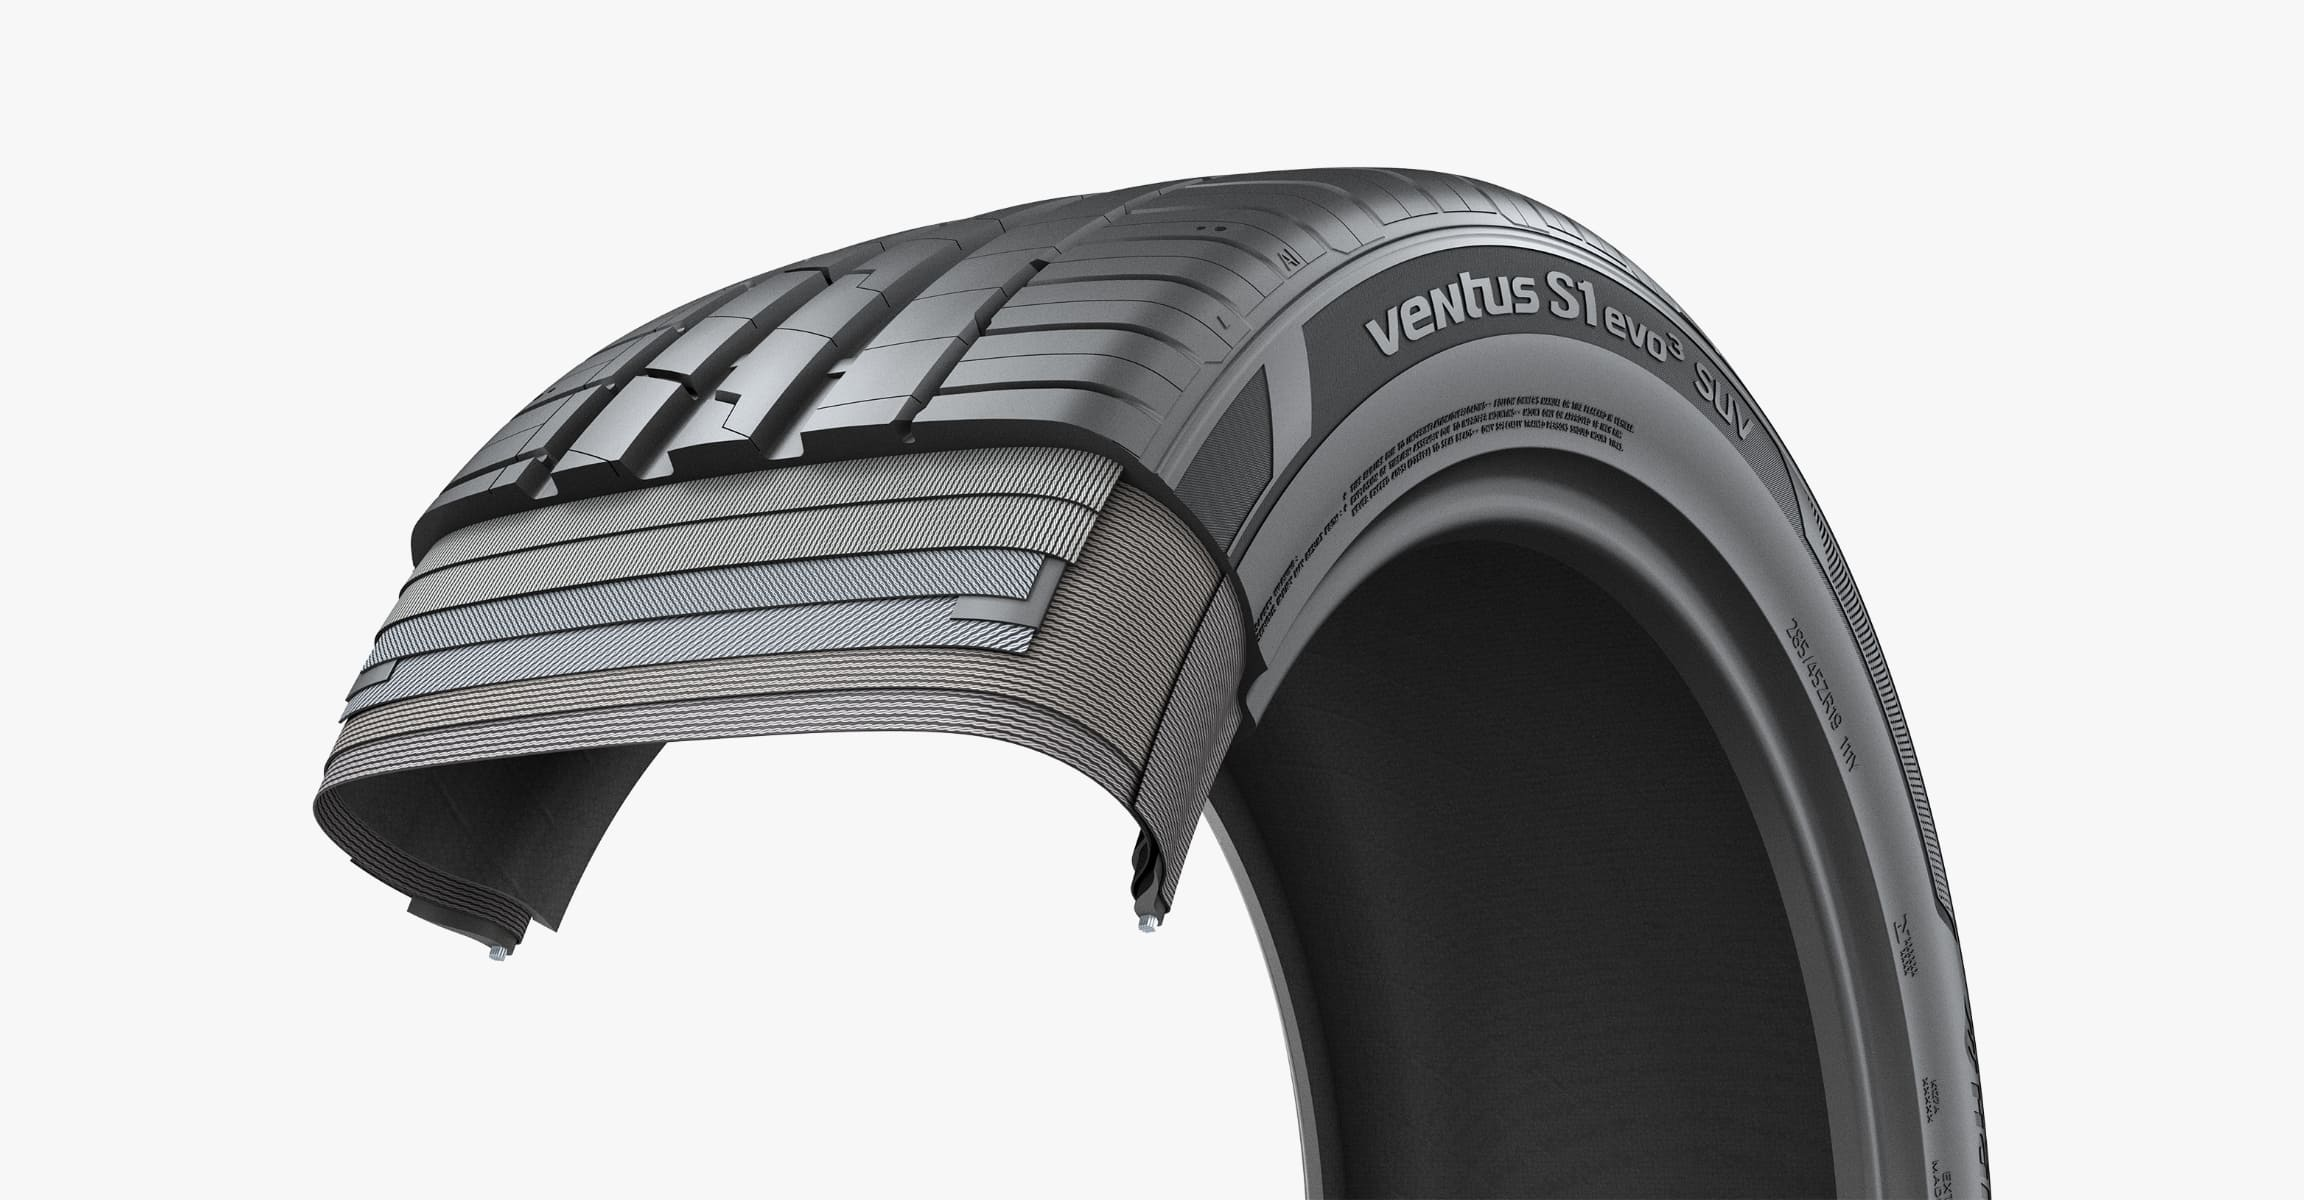
\includegraphics[scale=0.15]{Immagini/Tyres/Tire Structure_w.jpg}
    \caption{Struttura del pneumatico}
    \label{fig:Structure_tyres}
\end{figure}
\begin{description}
    \item[Carcassa :] è la parte più importante perchè rappresenta il telaio dello pneumatico. Il termine carcassa indica tutti gli strati composti dalle nappe a trama dello pneumatico. Assorbe la pressione dell'aria interna allo pneumatico, il peso e i colpi.
    \item [Strato intermedio e cintura :]
    è una struttura a nido d‘ape realizzata con fili di ferro collocata (diagonalmente) tra il battistrada e la carcassa, al fine di proteggere quest'ultima. Assorbe i colpi esterni e impedisce alle scheggiature o alle lesioni al battistrada di venire a diretto contatto con la carcassa. Allo stesso tempo, previene la separazione dello strato di gomma e della carcassa. La cintura ,invece, è un forte strato di rinforzo collocato nella circonferenza tra il battistrada e la carcassa negli pneumatici radiali e cinturati. Le funzioni della cintura sono simili a quelle dello strato intermedio; inoltre, rinforza la solidità del battistrada serrando saldamente la carcassa.
    \item [Spalla :] è la parte di pneumatico collocata tra il battistrada e la parete laterale, essa è composta dallo strato di gomma più spesso dell'intero pneumatico. Ha il compito di garantire la stabilità in curva e mantenere la traiettoria durante la guida.
    \item [Battistrada :] è composto da uno spesso strato di gomma che viene direttamente a contatto con la superficie stradale. È altamente resistente alla rottura e ai colpi, al fine di proteggere la carcassa e la cintura all'interno dello pneumatico. 
    il disegno dello stesso e la mescola di cui è composto sono caratteristica fondamentali che definiscono le prestazioni del pneumatico stesso .
    \item [Parete Laterale :] è collocata tra la spalla e il tallone, ha il compito di proteggere la carcassa e di aumenta le prestazioni di guida attraverso la sua flessibilità.
    \item [Tallone :] Ha il compito di fissare lo pneumatico al cerchione. È formato da varie parti, comprendenti il filo del tallone, il nucleo, la gomma e l'aletta. In generale, il cerchione è leggermente stretto, in modo che, in caso di riduzione improvvisa della pressione dell'aria durante la guida, lo pneumatico non si stacchi improvvisamente dal cerchione.
    \item [Liner interno :]
     consiste in uno strato di gomma con delle qualità ermetiche elevate. La gomma è generalmente composta di butile, da gomma sintetica o da un tipo di poli-isoprene. La funzione principale è quella di mantenere l'aria all'interno dello pneumatico.
\end{description}



\subsubsection{L'effetto del carico verticale}
La pressione media al suolo nell’area di contatto è, in prima approssimazione,
pari alla pressione di gonfiaggio del pneumatico

Il pneumatico, gonfiato ad una pressione p e soggetto ad un carico verticale $F_z$, si deformerà in modo tale da mettere in contatto con il suolo una superficie pari al rapporto $F_z / p$.
Questa deformazione comporterà uno schiacciamento pari ad f.
Più alto è il carico e più bassa è la pressione maggiore sarà la deformazione.

\subsubsection{Caratterizzazione dei pneumatici}
L'analisi del comportamento meccanico dei pneumatici si basa spesso sui risultati ottenuti sperimentalmente su singole gomme.\\
Per caratterizzare il pneumatico rispetto al comportamento direzionale si suppone che la superficie sia perfettamente piana e orizzontale.
Questo tipo di prove sono spesso svolte appoggiando la ruota su un tappeto mobile o su un tamburo rotante con superficie abrasiva.\\
Il sistema consiste in una macchina a disco rotante capace di misurare le forze e i momenti
agenti sullo pneumatico in seguito all’assegnazione di determinati valori di angoli di deriva,
di rollio e carico verticale.\\
Nonostante nessuna di queste prove standard corrisponde alle effettive condizioni di utilizzo i dati ottenuti sono comunque molto utili.
Essi sono di fondamentale importanza poichè nell'ultimo ventennio le simulazioni virtuali di veicoli sono diventate la base per la progettazione e l'ottimizzazione di veicoli.
Questi dati dovrebbero avere un accuratezza abbastanza elevata in modo da garantire una buona attendibilità delle simulazioni, con il passare degli anni sono stati sviluppati modelli empirici sempre più sofisticati in grado di avvicinarsi sempre maggiormente alla realtà.
Tuttavia non sempre i fornitori sono disposti a fornire dati accurati e completi per quanto riguarda i loro prodotti e spesso risultano difficili da reperire.

\subsection{Forze e slip}
Un pneumatico può essere descritto come un sistema in grado di generare forze e momenti come conseguenza degli input applicati.
\begin{figure}[ht]
    \centering
    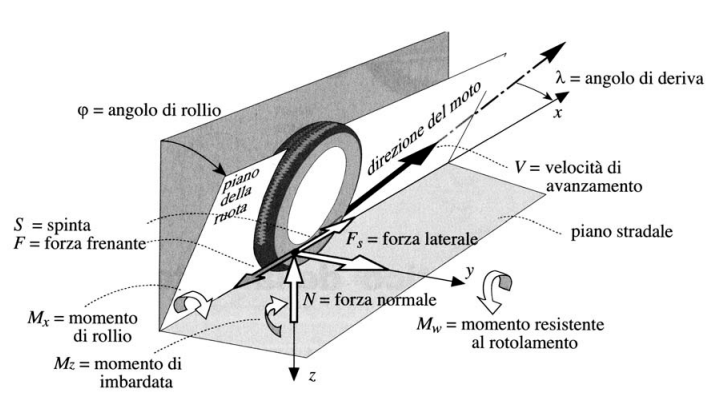
\includegraphics[scale=0.9]{Immagini/Tyres/tyre_forces.png}
    \caption{Forze e momenti generati dallo pneumatico}
    \label{fig:tyre_forces}
\end{figure}
Queste forze e momenti possono essere schematizzati come applicati in corrispondenza del centro del impronta a terra. Essi posso essere riassunti :
\begin{itemize}
    \item Una forza longitudinale, agente lungo la direzione x, assunta positiva in fase di
    accelerazione e negativa in fase di frenata. $\longrightarrow$ [$F_x$]
    \item Una forza laterale, orientata ortogonalmente a quella longitudinale ,direzione y, che garantisce la tenuta del veicolo. $\longrightarrow$ [$F_y$]
    \item Una forza normale al piano della strada, agente in direzione z. $\longrightarrow$ [$F_z$]
    \item Un momento di rollio attorno all’asse x. $\longrightarrow$ [$M_x$]
    \item Un momento di resistenza al rotolamento intorno all’asse y. $\longrightarrow$ [$M_y$]
    \item Un momento di imbardata intorno all’asse z. $\longrightarrow$ [$M_z$] 

\end{itemize}




\subsection{Magic Formula}
La Magic Formula è un modello empirico-matematico creato da Hans Bastiaan Pacejka, che che cerca di riassumere le prestazioni sperimentali dello pneumatico attraverso formule matematiche. Queste hanno una precisa struttura in cui compaiono coefficienti ricavati sperimentalmente e i parametri di funzionamento. L'obbiettivo è fornire in output varie forze e momenti che il pneumatico può generare.\\
La formulazione base è:
\begin{equation}
\label{eq:Pacjeka}
    y(x)=D*sin(C*arctant(Bx-E(Bx-arctan(Bx)))
\end{equation}
In questa formulazione la Y rappresenta la variabile in output desiderata, può essere
$F_x$, $F_y$ oppure $M_z$, $X$è la variabile in input scelta tra $\alpha$ e $k$. I Coefficenti B, C, D, E, chiamati anche coefficienti di Pacejka, esprimono:
\begin{itemize}
    \item B $\longrightarrow$ Stiffness factor \hspace{2.3cm} B $>$ 0
    \item C $\longrightarrow$ Shape factor \hspace{2.3cm} 1 $<$ C $<$ 2
    \item D $\longrightarrow$ Peak value  \hspace{2.6cm} D $= \mu*F_Z$
    \item E $\longrightarrow$ Curvature factor \hspace{2cm} E $<$ 1
\end{itemize}
I range consigliati sono presi da \cite{Guiggiani}.

\subsection{Evoluzione della Magic Formula}
La prima versione della Magic formula è stata sviluppata nel 1987 da allora sono state create una serie di nuove versioni.
Nel 1996 TNO automotive ha introdotto modello di pneumatico MF-Tyre 5.0 ed il software commerciale MF-Tool per l'estrapolazione dei parametri partendo dai dati sperimentali. Entrambi erano basati sulle equazioni presentate nell'articolo di Pacejka del 1996 \cite{Pacejka1997MagicFT}.\\ 
Nel corso degli anni sono stati apportati alcuni miglioramenti (es. aggiunta del
momento di ribaltamento, slittamento combinato migliorato, ecc.) e sono stati rilasciati i modelli: MF-Tyre 5.1 e MF-Tyre 5.2 seguentemente.\\ 
MF-Tyre è stato concepito specificatamente per autovetture e camion utilizzanti pneumatici con
angoli di inclinazione (camber) relativamente piccoli (fino a 10 gradi).\\
È stato necessario modificare le equazioni della MF, creando il modello MF-MCTyre 1.0 per poterlo utilizzare per i pneumatici delle moto che notoriamente lavorano con angoli di inclinazione molto più elevati. In una fase successiva si è migliorata la precedente versione rilasciando il MF-MCTyre 1.1.\\
Nella versione MF-Tyre 6.0 le equazioni sono state ri-adattate, in modo che un unico modello possa gestire sia i pneumatici per le auto che per le moto.
È stato aggiunto inoltre il turn slip per rappresentare, ad esempio, il momento di autoallineamento
che si verifica durante la sterzata del pneumatico a veicolo fermo.\\ 
La MF-Tyre 6.1 estende le equazioni per poter incorporare gli effetti delle variazioni nella pressione di gonfiaggio.\\
Nella MF-Tyre 6.2 il raggio di carico viene aggiornato per elevati angoli di deriva e camber. Rende inoltre disponibile l'estensione MF-Swift per motociclette. MF-Swift introduce un modello ad anello rigido, cioè si assume che la cintura del pneumatico si comporti come un corpo rigido. Questo comporta un attendibilità maggiore nella gamma di frequenze in cui la flessione della cintura del pneumatico può essere trascurata, a seconda del tipo di pneumatico siamo tra i 60 e i 100 Hz.\\ 
Il modello include gli effetti giroscopici ed utilizza un singolo punto di contatto per il calcolo dello slip; Riesce a descrivere lo slip in transitorio fino allo scorrimento completo, grazie al diminuzione della lunghezza di rilassamento all'aumentare dello slip. \\
MF-Swift è adatto per prove con raggi di curvatura che abbiano lunghezza d'onda dell'ordine di due volte la lunghezza del contatto.\\ 
\begin{figure}[!h]
    \centering
    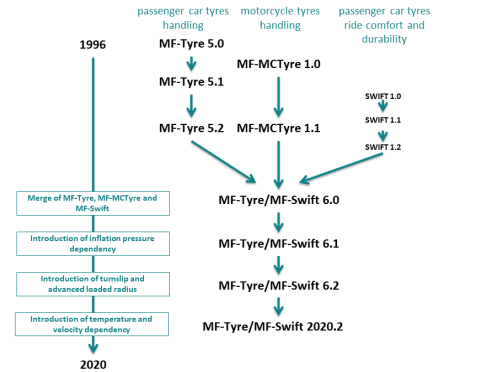
\includegraphics[scale=0.8]{Immagini/Tyres/MF-Tire History.png}
    \caption{}
    \label{fig:MF-Tire version history}
\end{figure}
\\
Per convenzione si utilizza una parola univoca che identifica la versione utilizzata è "FITTYP", questo parametro si trova nella sezione [model] del file.tir

\begin{itemize}
    {\tiny
    \setlength\itemsep{-0.5em}
    \item FITTYP = 5 \hspace{0.33cm} $\longrightarrow$ \hspace{0.2cm} MF-Tyre 5.0 , 5.1
    \item FITTYP = 6 \hspace{0.33cm} $\longrightarrow$ \hspace{0.2cm} MF-Tyre 5.2
    \item FITTYP = 21 \hspace{0.2cm} $\longrightarrow$ \hspace{0.2cm} 
    MF-Swift 1.1  (basato su MF-Tyre 5.2)
    \item FITTYP = 51 \hspace{0.2cm} $\longrightarrow$ \hspace{0.2cm} MF-MCTyre 1.0
    \item FITTYP = 52 \hspace{0.2cm} $\longrightarrow$ \hspace{0.2cm} MF-MCTyre 1.1
    \item FITTYP = 60 \hspace{0.2cm} $\longrightarrow$ \hspace{0.2cm} MF-Tyre 6.0
    \item FITTYP = 61 \hspace{0.2cm} $\longrightarrow$ \hspace{0.2cm} MF-Tyre 6.1
    \item FITTYP = 62 \hspace{0.2cm} $\longrightarrow$ \hspace{0.2cm} MF-Tyre 6.2
    \item FITTYP = 70 \hspace{0.2cm} $\longrightarrow$ \hspace{0.2cm} MF-Tyre 6.2 + Temperature and Velocity model

    }
\end{itemize}

\subsubsection{Tire property file}
Le versioni MF-Tyre precedentemente elencate sono modelli di simulazione di pneumatici definiti da una serie di parametri. Questi parametri vengono generalmente archiviati in dei file, chiamati "Tire Property File" aventi tipicamente l'estensione ".tir".\\ 
La figura \ref{fig:Structure_file_tir} mostra la classica struttura e il contenuto del file:\\
\begin{figure}[ht]
    \centering
    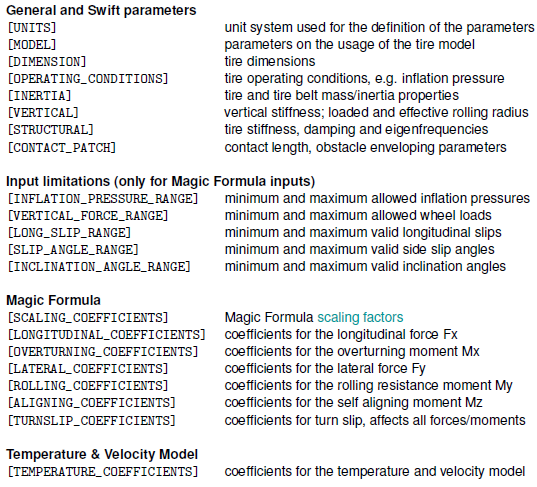
\includegraphics[scale=0.9]{Immagini/Tyres/Structure_file_tir.png}
    \caption{}
    \label{fig:Structure_file_tir}
\end{figure}
Nella prima sezione sono elencate tutte le informazioni generali , le unità di misura , tutte le caratteristiche geometriche del pneumatico
e le proprietà strutturali dello stesso.\\
Nella seconda sezione vengono elencati i limiti di pressione , forza verticale , slip e camber ai quali il modello può operare.\\
La terza sezione è la più ampia, all'interno si trovano numerosi coefficienti, di seguito elencheremo i più significativi.\\
I coefficienti di scala iniziano con la lettera L essi vengono inclusi nel file per poter ottenere un modello che simuli la realtà nel modo più affine possibile.
Come visto nell'introduzione ai pneumatici, le prove di forza e momenti vengono spesso eseguite in ambiente di laboratorio:\\ 
La superficie stradale artificiale della macchina di prova per pneumatici è usualmente molto diversa rispetto al reale manto stradale, questo, combinato all'incertezza sulla temperatura, umidità, usura, pressione di gonfiaggio, ecc., determina che il comportamento del pneumatico montato sul veicolo potrebbe discostarsi in modo significativo rispetto ai risultati ottenuti mediante la macchina di prova.\\
Verosimilmente si potrebbero avere differenze fino al 20$\%$ nel coefficiente di attrito e nella cornering stiffness \cite{Braghin2006EnvironmentalEO}.\\
I più importanti fattori di scala sono:\\
\begin{table}[h!] 
    {\scriptsize\setlength\itemsep{-0.2em}
    \centering
    \begin{tabular}{l l}
        \texttt{LMUX} \qquad \quad  & Scale factor of longitudinal peak friction coefficient\\
        \texttt{LKX} & Scale factor of longitudinal slip stiffness\\
        \texttt{LMUY} & Scale factor of lateral peak friction coefficient cornering stiffness\\
        \texttt{LKY} & Scale factor of cornering stiffness\\
        \texttt{LKYC} & Scale factor of camber stiffness\\
        \texttt{LTR} & Scale factor of pneumatic trail\\
        \texttt{LKZC} & Scale factor of camber moment stiffness\\
        \texttt{LMP} & Scale factor of parking moment at standstill\\
    \end{tabular}

    }
    \caption{}
    \label{tab:scaling factors}
\end{table}
\\
Nelle equazioni i coefficienti di scala vengono denominati attraverso il simbolo $\lambda$\\
I coefficienti della sezione 3 verranno discussi 
approfonditamente nelle successive sottosezioni.\\
La quarta sezione contiene i coefficienti per gli effetti termici e gli effetti di velocità.
Tuttavia essa si trova molto raramente per via della complessità che accompagna questi effetti.

\subsubsection{MF 5.2}
Fin dalla sua concezione, oltre 20 anni fa, la Magic Formula è stata adottata abbastanza rapidamente nell' industria come modello di pneumatico standard per simulazioni di manovrabilità dei veicoli.\\ 
Nel corso degli anni sono stati apportati vari sviluppi per
migliorare l'accuratezza ed estendere le capacità del modello.\\
Rispetto alla versione precedente (5.1), la 5.2 presenta alcune migliorie:\\
-I fattori di scala sono stati definiti in modo tale che gli effetti di conicità e plysteer possano essere facilmente disattivati.\\
-\'E stato introdotto il fattore "E", rendendo il modello più accurato in condizione di slip combinato (laterale + longitudinale).\\
-La resistenza al rotolamento è diventata funzione della velocità.\\
-Ed è stato introdotto l'effetto del Camber sul picco di forza longitudinale.\\

Il modello di pneumatico MF-Tyre 5.2 ha dimostrato una buona attendibilità ed è tuttora ampiamente utilizzato negli studi di dinamica dei veicoli. \\



Le equazioni del modello (si trovano nel MF-Tyre MF-5.2 users manual) \\
...................da completare.

\subsubsection{MF 6.1}
%Il modello MF-Tire 5.2 necessitava di alcune evoluzioni che ne ampliassero le potenzialità,
%gli obbiettivi erano:\\
Il modello MF-Tyre 6.1 rappresenta un evoluzione del 5.2, quest'ultimo infatti necessitava di alcune evoluzioni che ne ampliassero le potenzialità.\\
Nel 2010 il Dipartimento di ingegneria meccanica dell'Università di Eindhoven ha lavorato in tal senso con degli obbiettivi specifici:\\
-Migliorare la descrizione del camber, attraverso una formulazione ed un controllo espliciti sulla rigidezza al camber, estendendo inoltre le capacità del modello nel gestire angoli molto ampi (motocicli).\\
-Includere l'effetto della pressione di gonfiaggio. Questo permetteva di eliminare i numerosi file creati a diverse pressioni, in quanto consentiva di prevedere il
comportamento anche a pressioni differenti rispetto a quella con la quale si è svolto il test sperimentale, riducendo di conseguenza il numero di misurazioni richieste.\\
-Rendere coerente la descrizione della dinamica dei pneumatici tra MF-Swift e MF-Tire. Includendo l'effetto del rilassamento del pneumatico e della carcassa rigida.\\
-Migliorare la descrizione della resistenza al rotolamento e del momento di ribaltamento.\\

\begin{figure}[ht]
    \centering
    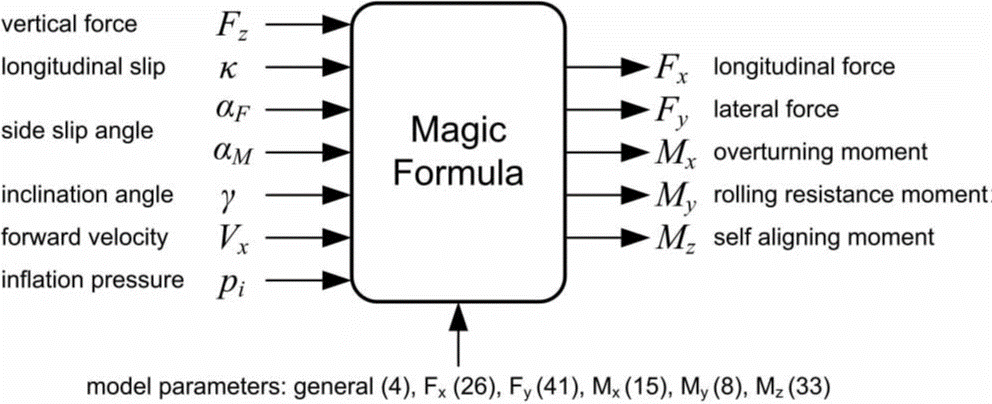
\includegraphics[scale=0.6]{Immagini/Tyres/MF.png}
    \caption{Input e output del modello MF-6.1}
    \label{fig:MF_tyres}
\end{figure}

\begin{figure}[ht]
    \centering
    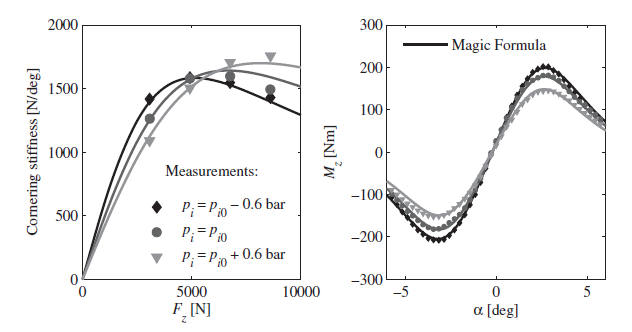
\includegraphics[scale=0.7]{Immagini/Tyres/Tyre pressure effects for a passenger car tyre.png}
    \caption{Effetto della pressione di gonfiaggio sulla cornering stiffness e sul momento di autollineamento}
    \label{fig:Pressure effects}
\end{figure}
La fig. \ref{fig:Pressure effects} mostra come al diminuire della pressione di gonfiaggio, la cornering stiffness aumenti in modo più rapido al crescere di $F_Z$ fino a valori di 5000[N] questo è dovuto al fatto .............\\
\begin{figure}[!h]
    \centering
    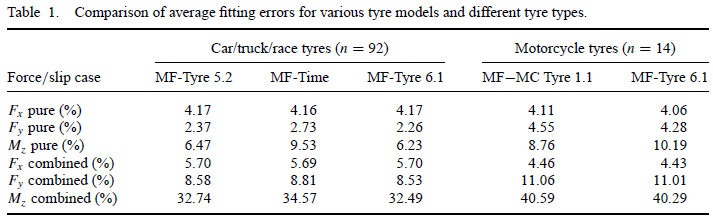
\includegraphics[scale=0.7]{Immagini/Tyres/comparison MF-Tire version.png}
    \caption{Confronto fra le versioni MF-Tire}
    \label{fig:Comparison MF-Tire version}
\end{figure}
La fig. \ref{fig:Comparison MF-Tire version} mostra un confronto tra la media degli errori di fitting.\\  
Le fig. \ref{fig:Pressure effects} e \ref{fig:Comparison MF-Tire version} sono prese da \cite{Besselink2010AnIM}.\\

\section{Dinamica Laterale} \label{Dinamica laterale}
In questo capitolo verranno descritte le basi della dinamica del veicolo per quanto concerne la dinamica laterale.\\
Il comportamento dinamico di un veicolo può essere suddiviso in: longitudinale (trazione
e frenata), laterale (handling) e verticale (comfort).
In questa trattazione ci occuperemo del comportamento laterale cioè l'insieme delle risposte dinamiche in direzione perpendicolare alla direzione del moto, che il veicolo restituisce in risposta agli input forniti dal guidatore (sterzo e velocità).\\
Le fonti di questo argomento sono \cite{Guiggiani} e \cite{limebeer2018dynamics}, mentre ulteriori approfondimenti si trovano in  \cite{pacejka2005tire}.\\



In questa prima analisi il veicolo viene considerato un unico corpo rigido in
moto su un piano, dunque avente tre gradi di libertà: due traslatori e uno
rotatorio con asse perpendicolare al piano considerato.\\ 
Per l'analisi (quasi)-stazionaria verranno utilizzati semplici modelli di veicoli. 


\subsection{Single track model}
Il modello a singola traccia anche chiamato impropriamente (in gergo) modello a "bicicletta" è il modello più semplice utilizzato per analizzare le dinamiche laterali dei veicoli.\\
\'E molto utile per comprendere i fenomeni di handling in quanto presenta il vantaggio dell'essere semplice ed intuitivo permettendo una rapida valutazione dell'influenza dei parametri caratteristici.\\
\begin{figure}[!h]
    \centering
    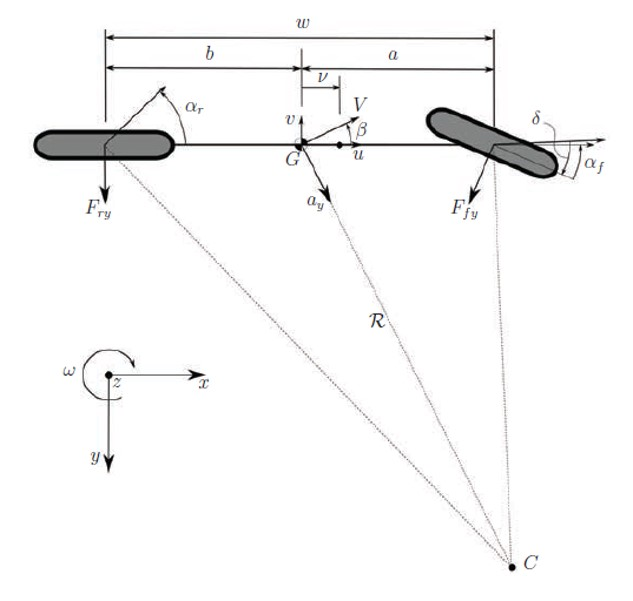
\includegraphics[scale=0.7]{Immagini/Lateral dynamics/Single_track_model.jpg}
    \caption{cinematica del single track model}
    \label{fig:Single track model}
\end{figure}
Ammettendo la simmetria rispetto all’asse longitudinale,
il veicolo può esser rappresentato da una sola linea con alle estremità i due
pneumatici (assale posteriore e anteriore sono condensati in due singole "
ruote equivalenti").\\
la fig. \ref{fig:Single track model} è la rappresentazione, appunto, della vista dall'alto di un veicolo privo di larghezza ,si tratta di un corpo rigido di massa $m$ concentrata nel centro di massa G, le cui distanze $a$ e $b$ sono i due semipassi,
rispettivamente anteriore e posteriore. Con $L$ o $W$ si indica il passo, cioè la distanza tra asse anteriore e posteriore.\\
%\singlespace 
Inoltre è possibile definire:
\begin{itemize}
    \begin{spacing}{1}
    \setlength\itemsep{-0.1em}
    \item \textbf{Velocità longitudinale} ($u$) : velocità di avanzamento in direzione longitudinale al veicolo.
    \item \textbf{Velocità laterale} ($v$) : velocità di scorrimento laterale del veicolo
    \item \textbf{Velocità d'imbardata} ($r$) : velocità angolare rispetto all'asse verticale z del sistema di riferimento assoluto
    \item \textbf{Angolo di assetto} ($\beta$) : angolo formato tra la direzione del vettore velocità assoluta e la direzione longitudinale del veicolo.
    \item \textbf{Angoli di deriva} ($\alpha_f$) e ($\alpha_r$) : angoli formati tra il piano medio della ruota (anteriore o posteriore) ed il vettore velocità del centro del impronta di contatto.
    \item \textbf{Angolo di sterzo} ($\delta$) : angolo formato tra l'asse di simmetria del veicolo ed il piano della ruota.
    \end{spacing}
\end{itemize}
Questo modello ignora gli effetti delle sospensioni, del telaio e del trasferimento del carico laterale.\\
\subsubsection{Equazioni di equilibrio}
La velocità assoluta del centro di massa può essere espressa attraverso i versori del sistema di riferimento del veicolo:\\
\begin{equation}
\textbf{V} = u\textbf{i}+v\textbf{j}
\end{equation}
L'accelerazione laterale è data:\\
\begin{equation}
\begin{split}
\frac{d\textbf{V}}{dt} & = \textbf{$\dot V$}+r\textbf{k}\times\textbf{V}\\
 & = \hat{a_x}\textbf{i}+\hat{a_y}\textbf{j}
\end{split}
\end{equation}
$\hat{a_x}$ è l'accelerazione longitudinale mentre $\hat{a_y}$ è accelerazione laterale normale al piano di simmetria del veicolo.\\
\begin{align}
\hat{a_x} & = \dot u - rv\\
\hat{a_y} & = \dot v + ru
\end{align}
Imponendo l'equilibrio delle forze in direzione longitudinale e laterale e dei momenti si ottengono le seguenti equazioni del moto:
\begin{align}
m(\dot u- rv) & = -F_{yf} \sin \delta+F_{xf} \cos \delta+F_{xr}\\
m(\dot v+ ru) & = +F_{yf} \cos \delta+F_{xf} \sin \delta+F_{yr}\\
J\dot r & = a*(F_{yf} \cos \delta+F_{xf} \sin \delta)-b*F_{yr}\\[3mm]
m\dot u & =  mrv-F_{yf} \sin \delta+F_{xf} \cos \delta+F_{xr} \label{eq:eom longitudinal}\\
m\dot v & = -mru+F_{yf} \cos \delta+F_{xf} \sin \delta+F_{yr} \label{eq:eom lateral}\\
J\dot r & = a*(F_{yf} \cos \delta+F_{xf} \sin\delta)-b*F_{yr} \label{eq:eom yaw}
\end{align}
Nelle quali $m$ e $J$ sono rispettivamente la massa ed il momento d'inerzia all'imbardata, mentre $u$, $v$, e $r$ sono le variabili di stato del modello.
Per veicoli a trazione posteriore (RWD) e ipotesi di resistenza al rotolamento nulla, la $F_{fx}$ è trascurabile.\\
Inoltre approssimando il $sin(\delta)=0$ e $cos(\delta)=1$, l'eq.\ref{eq:eom longitudinal} 
risulta disaccoppiata e dunque ininfluente nello studio delle dinamiche laterali\\
Rimangono di conseguenza solo le \ref{eq:eom lateral} e \ref{eq:eom yaw} che diventano:
\begin{align}
m\dot v & = -mru+F_{yf}+F_{yr}\label{eq:eom lateral 2}\\
J\dot r & = a*F_{yf}-b*F_{yr}\label{eq:eom yaw 2}
\end{align}

\subsubsection{Equazioni cinematiche}
I tre angoli di deriva possono essere calcolati utilizzando le seguenti relazioni cinematiche:
\begin{align}
\beta & = \arctan(\frac{v}{u})\\
\alpha_f & = \delta - \arctan(\frac{ra+v}{u})\\
\alpha_r & = \arctan(\frac{rb-v}{u})
\end{align}
Nell'ipotesi di piccoli angoli queste possono essere approssimate
\begin{align}
\beta & = \frac{v}{u}\\
\alpha_f & = \delta - \frac{ra+v}{u} \label{eq:alfa front} \\
\alpha_r & = \frac{rb-v}{u} \label{eq: alfa rear}
\end{align}
Definiamo con $R$ il raggio di curvatura : $R=\frac{u}{r}$.\\
Mentre la Curvatura è l'inverso del raggio di curvatura dunque $\rho = \frac{1}{R} = \frac{r}{u}$.\\
Attraverso l'equilibrio delle forze in direzione Z si ricavano i carichi verticali (statici) sui singoli assi:
\begin{align}
F_{zf} & = mg \frac{b}{a+b}\\
F_{zr} & = mg \frac{a}{a+b}
\end{align}

\subsubsection{Modello monotraccia lineare}
Si può riepilogare quanto visto finora attraverso il modello monotraccia lineare, Abbiamo visto nella sezione pneumatici come essi possano essere semplificati in modo puramente teorico con l' equazione costitutiva lineare dove la forza laterale generata è funzione dell'angolo di deriva moltiplicato per la rigidezza (cornering stiffness).
\begin{equation}
    \label{eq:Fy=C*alfa}
    F_{y,i} = C_i*\alpha_i
\end{equation}
Introducendo in quest'ultima equazione le equazioni cinematiche degli angoli di slip \ref{eq:alfa front} e \ref{eq: alfa rear} otteniamo:\\
\begin{align}
F_{yf} & = C_f*\alpha_f = C_f*(\delta - \frac{ra+v}{u}) \\
F_{yr} & = C_r*\alpha_r = C_r*(\frac{rb-v}{u}) 
\end{align}
Sostituendo queste due equazioni all'interno delle equazioni di equilibrio \ref{eq:eom lateral 2} e \ref{eq:eom yaw 2} otteniamo le seguenti equazioni del moto:
\begin{align}
m\dot v & = -mru + C_f\delta  + ( C_f - C_r)\frac{v}{u} + (- C_fa + C_rb)\frac{r}{u}\label{eq:eom lateral linear}\\
J\dot r & = aC_f\delta + (C_f a^2 + C_r b^2)\frac{r}{u} + ( C_fa - C_rb)\frac{v}{u}\label{eq:eom yaw linear}
\end{align}
\begin{align}
\dot v & = \frac{ C_f - C_r}{mu}v + \frac{- C_fa + C_rb}{mu}r - \frac{u}{m}r + \frac{C_f}{m}\delta\label{eq:eom lateral linear}\\
\dot r & = \frac{ C_fa - C_rb}{Ju}v + \frac{C_f a^2 + C_r b^2
}{Ju}r + \frac{aC_f}{J}\delta \label{eq:eom yaw linear}
\end{align}
In condizioni quasi-statiche le accelerazioni sono nulle dunque:
\begin{align}
0 & = \frac{ C_f - C_r}{mu}v + \frac{- C_fa + C_rb}{mu}r - ur + \frac{C_f}{m}\delta\\
0 & = \frac{ C_fa - C_rb}{Ju}v + \frac{C_f a^2 + C_r b^2}{Ju}r + \frac{aC_f}{J}\delta 
\end{align}
Questo è un sistema di due equazioni e due incognite $v$ e $r$ nel quale $u$ e $\delta$ sono gli input.\\
Introducendo la notazione matriciale il sistema \ref{eq:eom lateral linear} \ref{eq:eom yaw linear} può essere rappresentato attraverso le matrici A e B.\\
\begin{equation}
\begin{Bmatrix}
\dot v\\
\dot r
\end{Bmatrix}
=
\underbrace{\begin{bmatrix}
\frac{ C_f - C_r}{mu} & \frac{- C_fa + C_rb}{mu} - u\\
\frac{ C_fa - C_rb}{Ju}  & \frac{C_f a^2 + C_r b^2}{Ju} 
\end{bmatrix}}_{A}
\begin{Bmatrix}
v\\
r
\end{Bmatrix}+
\underbrace{\begin{bmatrix}
\frac{C_f}{m}\\
\frac{aC_f}{J} 
\end{bmatrix}}_{B}
\begin{Bmatrix}
\delta
\end{Bmatrix}
\end{equation}
In condizioni di regime ricaviamo la velocità laterale e la velocità angolare d'imbardata :
\begin{equation}
\begin{Bmatrix}
v\\
r
\end{Bmatrix}
=
\begin{bmatrix}
A 
\end{bmatrix}^{-1}
\begin{bmatrix}
B 
\end{bmatrix}
\begin{Bmatrix}
\delta
\end{Bmatrix}
\end{equation}

\subsubsection{Stabilità del modello}
Per lo studio della stabiità di marcia del modello è necessario analizzarlo in seguito ad una perturbazione rispetto alla condizione di equilibrio.
La risposta sarà una combinazione di modi di vibrare.
Un sistema è stabile quando i tutti suoi modi di vibrare hanno parte reale negativa, basta un singolo modo di vibrare con parte reale positiva e il sistema sarà instabile.\\
Le radici del polinomio caratteristico sono appunto i modi di vibrare.\\
Imponendo il $det[SI-A]=0$ troviamo gli autovalori:
\begin{gather}det
    \begin{bmatrix}
    S-\frac{ C_f - C_r}{mu} & \frac{ C_fa - C_rb}{mu} - u\\
    \frac{ -C_fa + C_rb}{Ju}  & S-\frac{C_f a^2 + C_r b^2}{Ju} 
    \end{bmatrix} = 0 \\
    \begin{bmatrix}
        S^2 - S\frac{C_f a^2 + C_r b^2}{Ju} - S\frac{C_f-C_r}{mu} + \frac{C_f-C_r}{mu}\frac{C_f a^2 + C_r b^2}{Ju}
    \end{bmatrix}
    -
    \begin{bmatrix}
        \frac{(C_fa-C_rb)^2}{mJu} + \frac{C_fa-C_rb}{J}
    \end{bmatrix} = 0\\
    \underbrace{\begin{bmatrix}
    1
    \end{bmatrix}}_{a_2}S^2 +
    \underbrace{\begin{bmatrix}
    \frac{C_f a^2 - C_r b^2}{Ju} + \frac{C_f+C_r}{mu}
    \end{bmatrix}}_{a_1} S +
    \underbrace{\begin{bmatrix}
    \frac{C_f-C_r}{mu}\frac{C_f a^2 + C_r b^2}{Ju} - \frac{(C_fa-C_rb)^2}{mJu} - \frac{C_fa-C_rb}{J}
    \end{bmatrix}}_{a_0} = 0
\end{gather}
Secondo il criterio di Hurwitz un sistema è stabile quando tutti i coefficienti del polinomio caratteristico hanno lo stesso segno.
Essendo $a_2$ e $a_1$ positivi, affinche il sistema sia stabile dovrà essere positivo anche $a_0$.
imponendo questa condizione otteniamo che affinchè il sistema sia stabile
\begin{equation}
    \begin{split}
        u^2 & < -\frac{C_f C_r (a+b)}{C_rb-C_fa} \frac{(a+b)}{m} \\
            & < -\frac{C_f C_r (a+b)}{mg(C_rb-C_fa)} (a+b)*g \\
          u & < \sqrt{-\frac{g(a+b)}{\zeta}}
    \end{split}
\end{equation}
Definiamo dunque la velocità critica valida solo per veicoli sovrasterzanti ($\zeta < 0$)
\begin{equation}
    u_{cr} = \sqrt{-\frac{g(a+b)}{\zeta}}
\end{equation}
Introduciamo ora il gradiente di sottosterzo per il modello lineare:
\begin{equation}
    \zeta = \frac{C_rb-C_fa}{C_f C_r (a+b)}*mg
\end{equation}
\begin{enumerate}
    \item Se $C_rb-C_fa < 0$ ($\zeta < 0$) il veicolo si definisce \textbf{sovrasterzante}
    \item Se $C_rb-C_fa = 0$ ($\zeta < 0$) il veicolo si definisce \textbf{neutro}
    \item Se $C_rb-C_fa > 0$ ($\zeta > 0$) il veicolo si definisce \textbf{sottosterzante}
\end{enumerate}
Ovvero se la capacità direttiva del retrotreno ($C_rb$) è maggiore della capacità direttiva dell'avantreno ($C_fa$) il
veicolo è detto sottosterzante in quanto il raggio di curvatura che percorre sarà maggiore del raggio di curvatura che 
dovrebbe percorrere dato dalla combinazione di velocità e angolo di sterzo. 
Questo argomento verrà trattato approfonditamente nel cap.\ref{cha:cap2}.

\subsection{Double track model}
Il modello a doppia traccia è l'evoluzione del modello a singola traccia, in questo caso il veicolo viene rappresentato attraverso la sua vista dall'alto con quattro ruote.\\
Questo modello permette di considerare gli effetti sul comportamento direzionale del trasferimento di carico laterale, della sterzata di Ackermann e toe, del camber e dell'aerodinamica.\\
Come nel caso precedente la dinamica longitudinale verrà trascurata in quanto non è argomento di tesi.\\

\begin{figure}[ht]
    \centering
    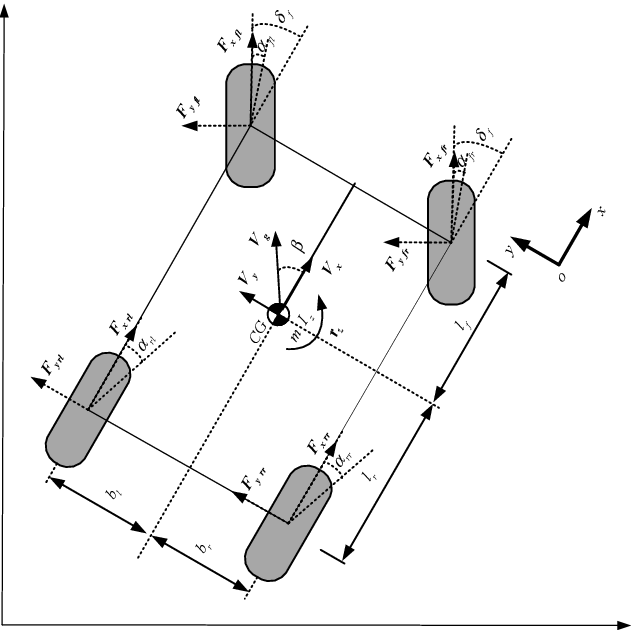
\includegraphics[scale=0.4]{Immagini/Lateral dynamics/Double-track-model-of-vehicle-lateral-dynamics.png}
    \caption{Double track model}
    \label{fig:Double track model}
\end{figure}
Come nel caso precedente possiamo scrivere le equazioni del moto: 
\begin{align}
\nonumber\\
m(\dot u- rv) & = F_{xrl} + F_{xrr} + F_{xfl} \cos \delta_l + F_{xfr} \cos \delta_r -F_{yfl} \sin \delta_l -F_{yfr} \sin \delta_r\\
m(\dot v+ ru) & = F_{yrl} + F_{yrr} + F_{yfl} \cos \delta_l + F_{yfr} \cos \delta_r +F_{xfl} \sin \delta_l +F_{xfr} \sin \delta_r\\
J\dot r & = a*(F_{yfl} \cos \delta_l + F_{yfr} \cos \delta_r +F_{xfl} \sin \delta_l +F_{xfr} \sin \delta_r)-b*(F_{yrl} + F_{yrr})
\end{align}
Ipotizzando $F_{xrl}=F_{xrr}$ le coppie differenziali posteriori sono nulle.\\
Gli angoli di deriva laterali risultano:\\
\begin{align}
\alpha_{fl} & = - (\frac{ra+v}{u+r\frac{Wt_{f}}{2}}) + \delta_f\\
\alpha_{fr} & = - (\frac{ra+v}{u-r\frac{Wt_{f}}{2}}) + \delta_r\\
\alpha_{rl} & = - (\frac{-rb+v}{u+r\frac{Wt_{r}}{2}})\\
\alpha_{rr} & = - (\frac{-rb+v}{u-r\frac{Wt_{r}}{2}})
\end{align}


\subsubsection{Trasferimento di carico laterale} \label{Trasferimento di carico laterale}
Per capire come i carichi verticali si ripartiscano durante una curva, si schematizza il veicolo come composto da tre corpi rigidi : massa sospesa, assale anteriore e assale posteriore.\\
La massa sospesa è vincolata a ciascun assale mediante una coppia rotoidale e le due coppie hanno asse coincidente, detto asse di rollio: 
è un asse parallelo all'asse longitudinale del veicolo individuato dalla retta che unisce i centri di rollio dell'asse anteriore e dell'asse posteriore.\\
La rotazione del veicolo attorno a quest'asse viene chiamata "rollio".\\
Il rollio avviene nei veicoli dotati di sospensioni durante una curva, a seguito della forza centrifuga generata, questa agendo sulla massa sospesa tende ad inclinarla nel direzione opposta rispetto alla direzione della curva.\\
La forza peso del veicolo tende ad aumentare nelle ruote esterne e diminuire nelle ruote interne.\\
\begin{align}
F_{zfl} & = mg \frac{b}{a+b} + m a_y \frac{h}{Wt_f} D + \frac{Faero_f}{2}\\
F_{zfr} & = mg \frac{b}{a+b} - m a_y \frac{h}{Wt_f} D + \frac{Faero_f}{2}\\
F_{zrl} & = mg \frac{a}{a+b} + m a_y \frac{h}{Wt_f} (1-D) + \frac{Faero_r}{2}\\
F_{zrr} & = mg \frac{a}{a+b} - m a_y \frac{h}{Wt_f} (1-D) + \frac{Faero_r}{2}
\end{align}
Definiamo con D il mechanical balance, un parametro che indica come si distribuirà il trasferimento di carico laterale tra assale anteriore e assale posteriore.
\begin{equation}
    D = \frac{K_{\phi f}}{K_\phi}\frac{h-d}{h} + \frac{b}{L} \frac{d_f}{h} \label{eq:Mechanical balance}
\end{equation}
Come si può vedere dall'eq.\ref{eq:Mechanical balance} questo parametro è funzione di :\\
$\bullet K_{\phi f}$ è la rigidezza torsionale dell'assale anteriore comprende le varie rigidezze delle sospensioni e delle eventuali barre di torsione presenti\\
$\bullet K_{\phi}$ è la rigidezza torsionale complessiva del veicolo, è la somma di $K_{\phi f}$ e $K_{\phi r}$.\\
$\bullet h$ è l'altezza del centro di massa rispetto al piano di appoggio.\\
$\bullet d_f$ è l'altezza del centro di rollio dell'asse anteriore.\\
$\bullet h$ è l'altezza del punto formato dall'intersezione tra l'asse di rollio e la retta verticale a distanza $a$ dall'asse anteriore.
\begin{figure}[ht]
    \centering
    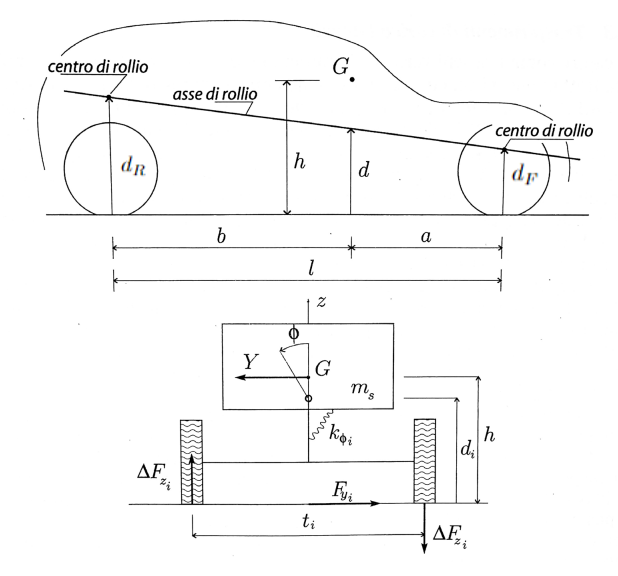
\includegraphics[scale=0.8]{Immagini/Lateral dynamics/Car roll 2.png}
    \caption{Vista laterale e frontale dello schema di veicolo}
    \label{fig:rollio}
\end{figure}


\subsubsection{Ackermann} \label{Ackermann}
Si definisce sterzata cinematica il moto di un veicolo lungo una traiettoria curva determinata dal puro rotolamento delle ruote.\\
In queste condizioni il centro di istantanea
rotazione O di tutte le ruote coincide: tale punto è anche il centro di curvatura 
dell’intero veicolo \ref{fig:Ackermann}.\\
\begin{figure}[ht]
    \centering
    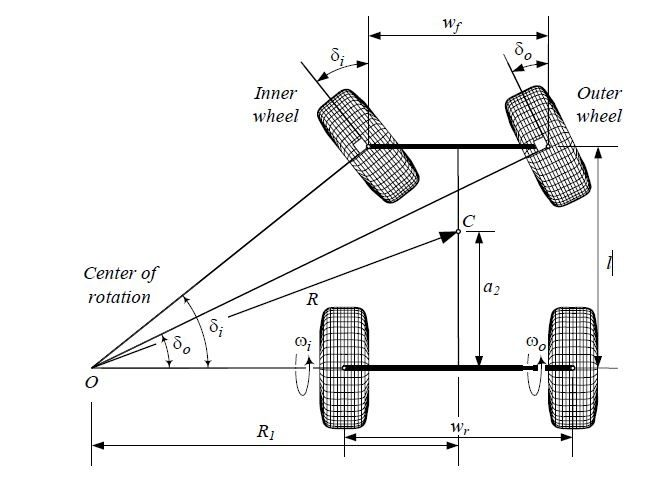
\includegraphics[scale=0.4]{Immagini/Lateral dynamics/Angolo-di-Ackermann.jpg}
    \caption{Sterzata di Ackermann}
    \label{fig:Ackermann}
\end{figure}
Affinchè il cir di tutte e 4 le ruote coincida, i due angoli di sterzo non possono essere uguali:
Le relazioni geometriche che descrivono le differenze tra i due angoli $\delta_{in}$ e $\delta_{out}$ possono essere facilmente ricavate dalla fig.\ref{fig:Ackermann}.\\
\begin{align*}
\tan(\delta_{in}) = \frac{l}{R-\frac{w_{tr}}{2}} &&  \tan(\delta_{out}) = \frac{l}{R+\frac{w_{tr}}{2}}
\end{align*}
Sottraendo le due otteniamo la "Relazione di Ackermann":
\begin{equation}
    \cot{(\delta_{out})} - \cot{(\delta_{in})} = \frac{w_{tr}}{l}
\end{equation}


\subsubsection{Camber} \label{Camber}
L'angolo di camber o "di campanatura" è l'angolo formato tra l'asse verticale passante per il centro dell'impronta di contatto dello pneumatico e l'asse radiale della ruota.\\
Se la parte superiore del pneumatico è più vicina alla macchina rispetto alla parte inferiore, il camber si considera negativo e viceversa.
Quando l'angolo di camber è nullo la superficie di contatto tra pneumatico e terreno sarà maggiore rispetto alle altre due configurazioni.
Si definisce camber statico è l'angolo misurato a veicolo fermo mentre il camber dinamico è funzione della cinematica delle sospensioni e dunque del trasferimento di carico.\\
Nelle auto da corsa è comune utilizzare un angolo di camber negativo, in quanto esso produce una forza laterale che migliora la tenuta in ingresso curva.

\begin{figure}[ht]
    \centering
    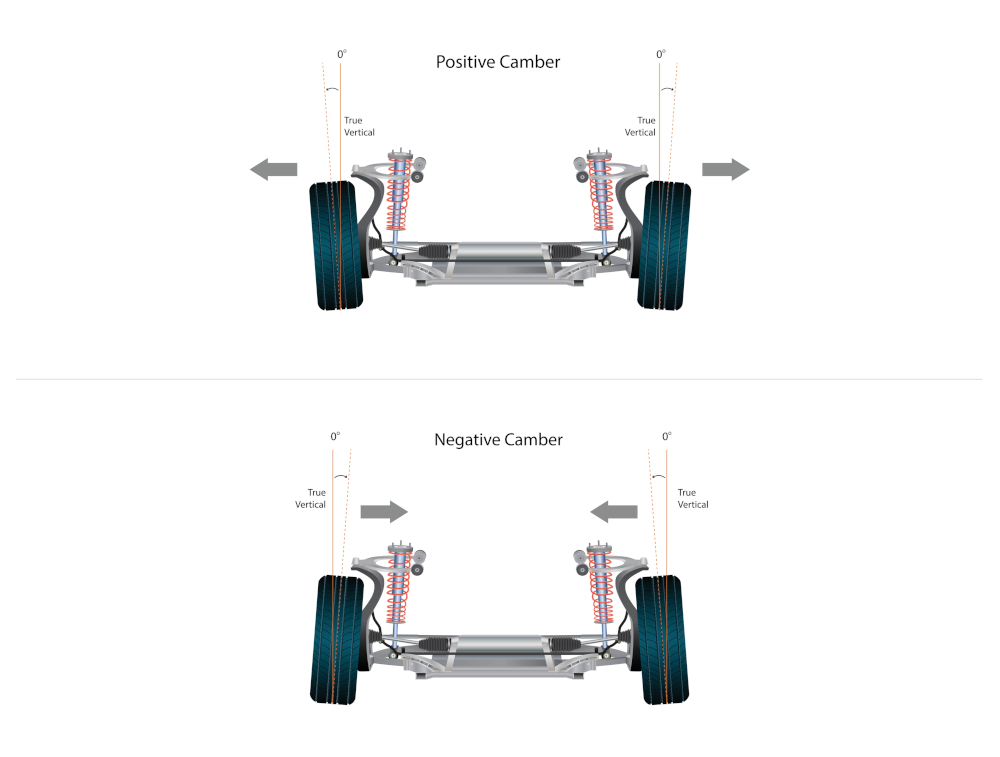
\includegraphics[scale=0.4]{Immagini/Lateral dynamics/Camber.jpg}
    \caption{Angoli di Camber}
    \label{fig:Camber}
\end{figure}


\subsubsection{Convergenza delle ruote} \label{Toe}
La convergenza delle gomme, chiamata anche "toe angle" è l'angolo che ogni rutoa forma con l'asse longitudinale del veicolo.\\
Quando l'angolo di toe è nullo le ruote sono parallele e puntano nella stessa direzione dell'asse longitudinale del veicolo.\\
\begin{figure}[ht]
    \centering
    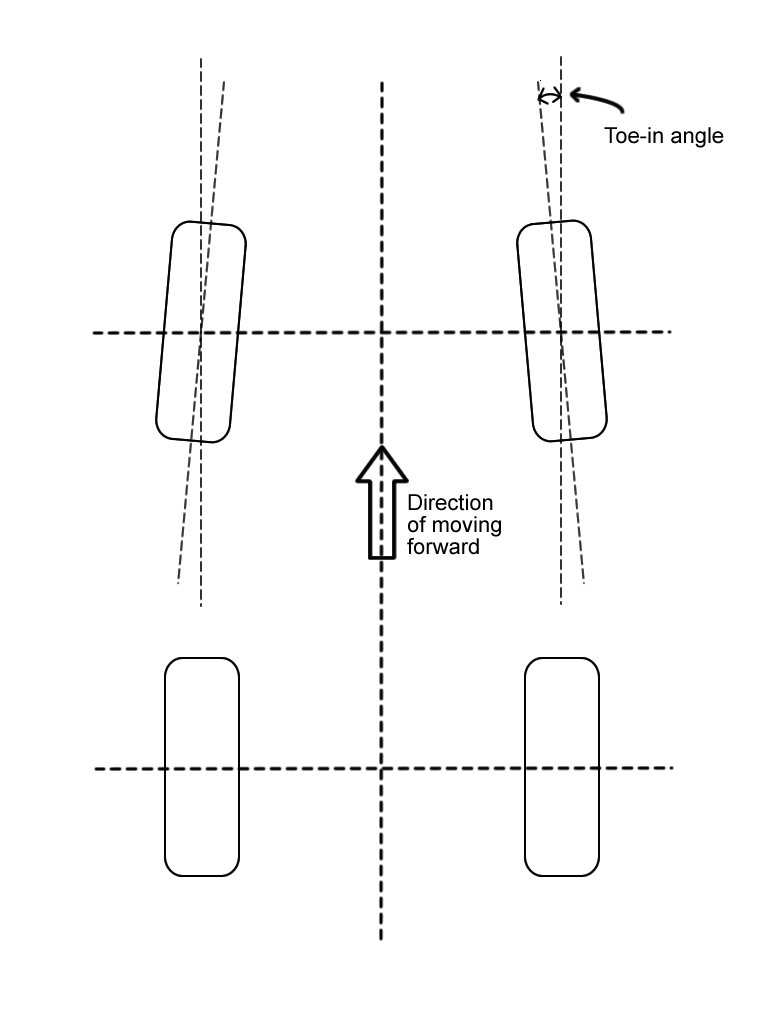
\includegraphics[scale=2]{Immagini/Lateral dynamics/Toe-in.png}
    \caption{Convergenza delle ruote anteriori}
    \label{fig:Toe-in}
\end{figure}
La convergenza delle gomme ha un forte impatto sulla stabilità del veicolo in rettilineo, sul comportamento in curva, ma anche sul consumo degli pneumatici e sulla loro temperatura di esercizio.\\ 
Utilizzando valori di convergenza positivi (toe-in), la vettura risulterà molto più stabile durante l'inserimento di curva aumentando il fenomeno del sottosterzo riducendo però la capacità direzionale dell'anteriore. \\
Al posteriore, il toe-in, favorisce una maggiore stabilità generale.\\
Viceversa, utilizzando “toe out” si avrà una vettura molto responsiva in fase di ingresso curva, ma meno stabile: all'aumentare del toe-out aumenterà il fenomeno del sovrasterzo.

\subsubsection{Aerodinamica}
I veicoli oltre a scambiare forze con il manto stradale tramite i pneumatici, interagiscono con l'aria, è importante capire come le forze aerodinamiche che nascono durante il moto influenzino il comportamento direzionale del veicolo.\\
Le forze aerodinamiche possono essere riassunte in due tipi:\\
$\bullet$ \textbf{Drag} (Resistenza all'avanzamento) : è la forza orizzontale agente sul centro di pressione che si oppone al moto del veicolo.\\
$\bullet$ \textbf{Down force} (Deportanza / Portanza) : è la forza verticale che nel caso delle autovetture è opposta al verso della forza peso, mentre nelle vetture da corsa ha lo stesso verso della forza peso ed è di fondamentale importanza per la prestazione in curva delle stesse.\\
L'efficienza aerodinamica di una vettura da corsa rappresenta appunto la capacità di generare deportanza riducendo al minimo la resistenza all'avanzamento.
A queste si aggiunge anche una Forza aerodinamica laterale $F_{ay}$.\\
Com'è noto le forze aerodinamiche dipendono dal quadrato della velocità:\\
\begin{align*}
F_{ax} = \frac{1}{2}\rho S C_x u^2 &&  F_{ay} = \frac{1}{2}\rho S C_y u^2 &&  F_{az} = \frac{1}{2}\rho S C_y u^2\\
\end{align*}
\chapter{Il Gradiente di sottosterzo}
\label{cha:cap2}
Una classica caratteristica del comportamento in curva di un veicolo, è il concetto di
sottosterzo, sovrasterzo o sterzo neutro (introdotto nella sez.\ref{Dinamica laterale}).\\
Si può esprimere questo concetto (in modo semplice) basandosi sull’interazione tra la velocità di avanzamento e la curvatura durante la percorrenza di una curva in condizioni stazionarie:\\
Se all’aumentare della velocità del veicolo cresce la curvatura percorsa allora 
siamo in condizione di sottosterzo.
Quando la curvatura rimane invariata all’aumentare della velocità allora siamo in
condizione di sterzo neutro.\\
Per lo studio della stabilità direzionale dei veicoli era necessario avere un indicatore intuitivo che descrivesse le differenze tra i casi elencati;\\ 
Il gradiente di sottosterzo è un parametro chiave utilizzato per quantificare e comprendere questo comportamento.\\
Questo concetto è stato introdotto per la prima volta da Olley nel 1946 \cite{Olley1946RoadMO}:\\
-Olley definì la "Linea di sterzo neutro" come il punto dove qualsiasi forza esterna applicata non produce alcun momento d'imbardata addizionale durante una curva ed Il gradiente di sottosterzo sarà dunque la distanza longitudinale tra il centro di massa e la linea di sterzo neutro.
Sebbene non siano state ricavate espressioni matematiche questo concetto coinvolge le derivate degli angoli di deriva dei pneumatici.\\
-A seguito dell'introduzione della sterzata cinematica (Ackermann), fù proposta un nuova formulazione definita come la differenza tra l'angolo di sterzo di riferimento e l'angolo di sterzo cinematico : $Ua_y = \delta_{REF} - \delta_A$ \cite{society1965vehicle}.\\
-Nel 1973 Pacjeka, studiò il concetto di gradiente di sottosterzo, scrivendo l'articolo \cite{doi:10.1080/00423117308968439}, nel quale presentava un metodo approssimato che permetteva di
creare un diagramma (handling diagram) utile per analizzare la stabilità in curva di un veicolo 
stradale in condizioni stazionarie.\\
Nella seconda parte dell'articolo \cite{doi:10.1080/00423117308968440} dimostrò, utilizzando il modello a singola traccia linearizzato ed esaminandone i poli, come il sottosterzo garantisca la stabilità in curva in condizioni stazionarie.\\
-Nel 1996 tramite lo standard SAE \cite{J266_201811}, si definirono le procedure per i test di controllo direzionale dei veicoli stradali, in modo da considerare le varie possibili condizioni di prova. \\
Furono apportate,inoltre, delle migliorie nella formulazione basata sulla sterzata cinematica, aggiungendo la possibilità di includere lo sterzo posteriore, in questo caso l'angolo di riferimento è dato dalla differenza tra l'angolo di sterzo anteriore e posteriore.\\
-Recentemente Guiggiani formulò delle perplessità riguardanti le definizioni del gradiente di sottosterzo esistenti, sostenendo che fossero chiaramente definite per veicoli a 4 o più ruote.\\
In un primo momento propose un miglioramento del $K_{SAE}$ per renderlo indipendente dal passo dei veicoli.
Successivamente propose un nuovo approccio all'handling che analizzeremo in seguito.

\section{Formulazioni classiche del gradiente di sottosterzo}
Le tre formulazioni maggiormente utilizzate sono: $K_{Pacejka}$ , $K_{SAE}$ , $K_{Guiggiani}$.
\subsection{Formulazione di Pacejka}

\subsection{Formulazione SAE}

\subsection{Formulazione di Guiggiani}

\subsection{Confronto e limiti delle formulazioni classiche}
Non sono ben definiti nei punti di flesso ecc ecc

\section{Formulazioni alternative del gradiente di sottosterzo}
\subsubsection{Bucchi e Frendo}

Le formulazioni classiche concentrano l'attenzione sul controllo dell'imbardata del veicolo utilizzando modelli fortemente semplificati sia per i pneumatici che per la dinamica del veicolo.\\
La nuova formulazione proposta nell'articolo \cite{doi:10.1080/00423114.2016.1167225} mette in relazione  il gradiente di sottosterzo alla coppia d'imbardata, a partire da manovre quasi stazionarie facilmente eseguibili su veicoli reali.\\
Questa formulazione si basa sulla conoscenza della derivata (rispetto al tempo) della curvatura e del momento d'imbardata generato dalle forze dei pneumatici.\\

(Partiamo dalle mappe di Guiggiani)
Poiché è dispendioso ottenere le mappe per tutte le combinazioni di $\Tilde{a_y}$ e $\delta_W$, si considerano manovre a velocità costante ($\dot{u} = 0$) e ($\dot{\delta_W} =$ costante) per ottenere informazioni sul comportamento dinamico del veicolo considerato. Queste manovre possono essere considerate rappresentative (con buona approssimazione ) delle comuni azioni di guida.\\
A partire dalla mappa $\rho_p(\Tilde{a_y}, \delta_W)$, si può scriverne il differenziale:
\begin{equation}
   d\rho_p = \frac{\partial \rho_p}{\partial \Tilde{a_y}} d\Tilde{a_y} + \frac{\partial \rho_p}{\partial \delta_W} d\delta_W 
\end{equation}
Se $\delta_W(t)$ varia lentamente e $u = \text{costante}$ allora: \quad $\rho \approx \rho_p$ \quad e \quad  $a_y = \dot{\beta}u + \rho u^2 - \tilde{a}_y$.\\ 
In questo caso, le "steady-state map" ($\beta_p$ , $\rho_p$) possono comunque essere utilizzate per valutare la derivata della curvatura $\dot{\rho}$ a partire dal differenziale $d\rho_p$ come segue:
\begin{equation} \label{17}
\dot{\rho} \cong \frac{\partial \rho}{\partial \tilde{a}_y} \dot{a}_y + \frac{\partial \rho}{\partial \delta_w} \dot{\delta}_w = - \frac{K}{l}\dot{a}_y + \frac{\tau}{l} \dot{\delta}_w
\end{equation}
Questa espressione non è generale e può essere considerata corretta solo nelle condizioni in cui la $\dot{\delta_W}$ sia relativamente bassa e $\beta$,$\rho$ possano essere approssimate dalle steady-state maps.\\
Il termine $\dot{a}_y$ può essere ottenuto a partire dalla definizione di accelerazione laterale per manovre a velocità costante:
\begin{equation} \label{18}
    \dot{a}_y = \frac{d(\dot{\beta}u + \rho u^2)}{dt} = \ddot{\beta}u + \dot{\rho}u^2 \cong \dot{\rho}u^2
\end{equation}
dove $\dot{u} = 0$   e  $\ddot{\beta}u \approx \dot{\rho}u^2$ (in condizioni di guida standard).\\ 
Sostituendo l'Eq. \ref{18} nell'Eq. \ref{17}, si ottiene una nuova definizione del gradiente di sottosterzo:
\begin{equation} \label{19}
    K \cong \frac{1}{u^2} \left( \frac{\tau \dot{\delta}_w }{\dot{\rho}} - l \right)    
\end{equation}
che può essere scritto in modo alternativo come una funzione del momento d'imbardata $N$:
\begin{equation} \label{20}
    K \cong \frac{1}{u^2} \left( \frac{\tau \dot{\delta}_wJu}{N} - l \right)
\end{equation}
%L'eq. \ref{19} consente di valutare il gradiente di sottosterzo sulla base di $\dot{\delta}_W$ e $\dot{\rho}$, misurabili attraverso un encoder sul volante e due accelerometri in due posizioni diverse del veicolo. \\
L'efficacia dell'eq.\ref{19}, deriva dal fatto che $K$ possa essere ricavato sperimentalmente eseguendo manovre quasi-stazionarie a velocità costante, misurando facilmente $\dot{\delta}_W$ e $\dot{\rho}$ attraverso un encoder sul volante e due accelerometri in due posizioni diverse del veicolo. \\
Se la velocità del volante $\dot{\delta}_W$ viene mantenuta costante, il momento d'imbardata è inversamente correlato al gradiente di sottosterzo (\ref{20}):\\ 
All'aumentare del momento d'imbardata, $K$ diminuisce $\xrightarrow{}$ il veicolo diventa più sovrasterzante.\\
Nel caso $N = 0$ possono verificarsi tre circostanze:\\ 
$\bullet$ Se $\dot{\delta}_W = 0$ l'eq. \ref{20} è indeterminata, tuttavia essendo in condizioni stazionarie possiamo calcolare il gradiente di sottosterzo con la formulazione classica.\\
$\bullet$ Se $\dot{\delta}_W \neq 0$, $K$ tende all'infinito, significa che la curvatura non varia nonostante la velocità di rotazione del volante sia diversa da zero.\\
In particolare,
se $\dot{\delta}_W > 0$ si verifica il sottosterzo poiché la velocità d'imbardata del veicolo non aumenta anche se il conducente sta aumentando l'angolo di sterzo.\\ 
Al contrario, se $\dot{\delta}_W < 0$ si verifica il sovrasterzo poiché la velocità d'imbardata del veicolo rimane costante anche se il conducente sta controsterzando.\\
% L'equazione \ref{20} è molto importante poiché apre la possibilità di controllare attivamente la virata del veicolo, 
attraverso lo sviluppo del torque vectoring, 
in quanto collega la definizione classica del sottosterzo al momento d'imbardata.
\section{Nuovo approccio all'handling}


\section{Metodi per la misura del sottosterzo}
\subsection{ISO-4138-2021}
La normativa ISO 4138 specifica metodi di test "open loop" per determinare il comportamento direzionale di autovetture stradali (ISO 3833) e di camion leggeri.\\
Il comportamento direzionale riguarda la dinamica del veicolo in generale e la "tenuta di strada"
Le manovre "open loop" descritte in seguito non sono rappresentative delle condizioni reali di guida, ma sono comunque molto utili per ottenere misure del comportamento complessivo del veicolo a seguito di diversi tipi di input di controllo e sotto condizioni di prova rigidamente definite.
I tre metodi definiti dalla normativa \cite{iso4138} sono:
\begin{enumerate}
    \item "Costant-speed test method"
    \item "Costant-steering-wheel angle test method"
    \item "Costant-radius test method"
\end{enumerate}
\subsubsection{Costant-speed test method}
Questo metodo di prova prevede che il veicolo sia condotto con velocità velocità costante variando l'angolo di sterzo.\\
Le caratteristiche direzionali sono determinate dai dati ricavati rispetto all'accelerazione laterale ma potrebbe
richiedere ampie aree di test, a seconda della combinazione di velocità e accelerazione laterale. \\
La variazione dell'angolo di sterzo dovrebbe essere più accurata possibile per garantire affidabilità dei dati.\\
La velocità di riferimento della prova è 100 [km/h], ma possono essere eseguite prova a diverse velocità.\\
Viene comunemente chiamato "rampsteer" (rampa di sterzo).\\
\subsubsection{Costant-steering-wheel angle test method}
Questo metodo di prova prevede che il veicolo sia condotto con velocità velocità crescente ed un angolo di sterzo mantenuto fisso.\\ 
Il raggio percorso sarà funzione della velocità di avanzamento e dell'accelerazione laterale.\\
Il test può essere eseguito con una serie di prove discrete oppure con una singola prova continua.\\
Nella prima, l'angolo dello sterzo viene applicato con il veicolo che viaggia a velocità discrete e viene mantenuto fino a quando non si raggiungono condizioni stazionarie.\\ 
Nella seconda, l'angolo dello sterzo viene mantenuto fisso mentre la velocità aumenta in modo lento e continuo fino al limite di controllo.\\
L'angolo di sterzo dovrà fornire un raggio percorso a bassa velocità di almeno 30 [m] e minimo 20 [m] valore limite.\\
Viene comunemente chiamato "rampspeed" (rampa di velocità).
\subsubsection{Costant-radius test method}
Questo metodo di prova prevede che il veicolo sia condotto a diverse velocità su un percorso circolare di raggio definito. Il raggio di curvatura di riferimento è solitamente 100 [m], possono essere utilizzati raggi maggiori e minori, Viene raccomandato un valore minimo di 40 [m]. \\
Le caratteristiche di risposta direzionale sono determinate attraverso i dati ottenuti.\\
Questa procedura può essere condotta in un'area relativamente piccola risultando adatta alle strutture esistenti nel quale
possa essere individuata una circonferenza sufficientemente ampia, può essere svolta in due varianti: \\
-Nella prima il veicolo percorre un percorso circolare a velocità discrete e costanti. 
I dati vengono rilevati quando viene raggiunto lo stato stazionario. 
Il test può essere eseguito su qualsiasi percorso livellato a raggio costante di lunghezza sufficiente per raggiungere e 
mantenere lo stato stazionario a raggio costante per almeno un periodo di misurazione di 3 s.\\
-Nella seconda, il veicolo rimane sul cerchio con un continuo e lento aumento di velocità, durante il quale vengono
rilevati i dati. La derivata dell'accelerazione laterale dovrebbe essere di 0,1 [m/s²/s] con un limite massimo di [0,2 m/s²/s].



\chapter{Simulazioni in ambiente Matlab}
\label{cha:cap3}
In questo capitolo verrà descritta l'implementazione tramite software matlab dei modelli descritti nel capitolo \ref{cha:cap1}, successivamente verranno esposti attraverso la rappresentazione dei risultati gli effetti sul comportamento direzionale dei parametri descritti nelle sez. \ref{Camber}.
%--------------------------------------------------------------------------------------------------------------
\section{Implementazione Steady state system}

\subsection{Single track model}

\subsection{Double track model}
\subsubsection{Load transfer}

\subsection{Functions}

\subsubsection{MFeval}
\subsubsection{Ackermann}
\subsubsection{-----------------------------}

%-----------------------------------------------------------------------------------------------------
\section{Descrizione Test}
$\bullet$\textbf{Manovra quasi-stazionaria} : Si osservano condizioni di regime successive, dunque non si considera la variabile tempo; 
il risultato sono i valori di regime ($v,r$) in funzione di uno o più parametri quali ($\delta,u$).\\
$\bullet$\textbf{Manovra dinamica} : Il sistema veicolo evolve nel tempo in base alle condizioni iniziali e ai comandi imposti dal guidatore (sterzo e velocità di avanzamento), 
il risultato sono le funzioni del tempo $v(t),r(t)$ delle variabili di stato.\\


\subsection{Rampsteer}
é una prova che prevede un test con angolo di sterzo crescente partendo da un angolo di sterzo alle ruote di 0 [deg] a 15 [deg].
Nel mentre si mantiene costante la velocità.
Per ogni test di rampsteer si eseguono 4 diverse prove a velocità di 30 - 60 - 90 - 120 [km/h].

\subsection{Costant steer}
é una prova che prevede un test a velocità longitudinale crescente partendo da una velocità di 0 [km/h] a 120 [km/h].
Nel mentre si mantiene costante l'angolo di sterzo alle ruote.
Per ogni test di costant steer si eseguono 4 diverse prove ad angolo di sterzo alle ruote di 5 - 10 - 15 - 20 [deg].

\subsection{Costant radius}
Questo metodo di prova prevede  veicolo a diverse velocità su un percorso circolare di raggio noto. Il raggio standard del percorso deve essere di 100 m, ma possono essere utilizzati raggi maggiori e minori, con 40 m come valore inferiore raccomandato e 30 m come minimo.
Le caratteristiche di risposta del controllo direzionale sono determinate dai dati ottenuti durante la guida del veicolo a velocità crescenti sul percorso di raggio costante. Questa procedura può essere condotta in un'area relativamente piccola. La procedura può essere adattata alle strutture esistenti selezionando un cerchio o un percorso di raggio appropriato.
\\Questa prova può essere svolta in due varianti. Nella prima il veicolo percorre un percorso circolare a velocità discrete e costanti. I dati vengono rilevati quando viene raggiunto lo stato stazionario. Il test può essere eseguito su qualsiasi percorso livellato a raggio costante di lunghezza sufficiente per raggiungere e mantenere lo stato stazionario a raggio costante per almeno un periodo di misurazione di 3 s. Nella seconda, il veicolo rimane sul cerchio con un continuo e lento aumento di velocità, durante il quale vengono rilevati i dati.
\\Nel nostro caso prevede un test a velocità longitudinale crescente partendo da una velocità di 0 [km/h] a 120 [km/h].
Nel mentre si mantiene costante il raggio di curvatura.
L'angolo di sterzo variabile sarà un output del sistema.

\subsection{Equivalenza tra i 3 metodi utilizzati}
La natura di qualsiasi stato stazionario stabile è indipendente dal metodo con cui viene raggiunto. Pertanto, per ottenere
un insieme  di condizioni di equilibrio di velocità, angolo di sterzo e curvatura, è possibile mantenere costante uno di
essi, variare il secondo e misurare il terzo.\\ 
Per definizione di sistema stazionario uno stato di equilibrio non è influenzato dallo stato di equilibrio precedente ed i
suoi parametri non dipendono dal tempo. 
In questo modo tutti i metodi di prova possono essere utilizzati, Questo trova pieno riscontro nelle simulazioni eseguite:\\

\section{Effetto dei parametri caratteristici}


\chapter{Effetti del modello matematico nella simulazione}
\label{cha:cap4}


In questo capitolo verranno descritti i risultati delle 
simulazioni matlab, evidenziando le differenze che si verificano
sulla base del modello matematico utilizzato per la simulazione.

\section{Alfa Romeo Giulia}
Le simulazioni sono state eseguite utilizzando i dati della 
Alfa Romeo Giulia 2.2 Turbodiesel 150 cv.
I dati sono stati presi da un modello VI-grade presente nei 
database unipd in modo tale da poterne confrontare i risultati.

\subsection{Parametri geometrici}
\begin{table}[H]
    \centering
    \caption{Main vehicle parameters}
    \vspace{0.5em}
    \begin{tabular}{ccc}
    \hline
        Symbol & Name and unit & Value\\
        \hline
        m & Mass [kg] & 1449\\
        J & Moment of inertia of yaw motion [kg $m^2$] & 2129 \\
        l & Wheelbase [m] & 2.82\\
        a & Front semi-wheelbase [m] & 1.315\\
        b & Rear semi-wheelbase [m] & 1.505\\
        $\tau$ & Transmission ratio & 11.8\\
        $W_f$ & Front wheel track [m] & 1.557\\
        $W_r$ & Rear wheel track [m] & 1.625\\
        h & Center of mass height [m] & 0.592\\
        $d_f$ & Front roll center height [m] & 0.041\\
        $d_r$ & Rear roll center height [m] & 0.086\\
    \hline    
    \end{tabular}
    \label{tab:tabella parametri Giulia}
\end{table}

\subsection{Rigidezze}
\begin{table}[H]
    \centering
    \caption{Roll stiffness}
    \vspace{0.5em}
    \begin{tabular}{ccc}
    \hline
        Name & Value & Unit \\
        \hline
        Front suspension stiffness & $20.8*10^3$ & [N/m]\\
        Front rollbar stiffness & $4.168*10^4$ & [Nm/rad]\\
        Rear suspension stiffness & $28.8*10^3$ & [N/m]\\
        Rear rollbar stiffness & $1.1709*10^4$ & [Nm/rad]\\
        Roll stiffness ratio & 0.6468 & [-]\\
    \hline    
    \end{tabular}
    \label{tab:tabella rigidezze}
\end{table}

\subsection{Pneumatici}
Per le simulazioni dei file.tir forniti da Pirelli riguardanti dei pneumatici ----- e -----
e dei pneumatici Toyo del tipo...

\section{Confronti}
I risultati mostrano che Utilizzando il modello single track
indipendentemente dalla prova utilizzata i risultati sul 
gradiente di sottosterzo sono analoghi.
Aumentando la complessità del modello si riscontrano delle differenze

\chapter{Simulazioni multibody}
\label{cha:cap5}
La simulazione multicorpo (MBS) è un metodo di simulazione numerica in cui i sistemi multicorpo sono composti da vari corpi. I corpi possono essere sia rigidi che elastici e le loro connessioni vengono modellate con vincoli cinematici (come giunti) o elementi di forza (come ammortizzatori a molla).

La simulazione multibody è uno strumento utile per condurre l'analisi del movimento.

Il cuore di qualsiasi programma software di 
simulazione multibody è il risolutore .
Il risolutore non è altro che un insieme di 
algoritmi di calcolo che risolvono le equazioni del moto arrivando alla descrizione cinematica.\\
L’analisi multi-corpo (multi-body) permette di simulare il comportamento 
cinematico, dinamico e strutturale di assiemi meccanici composti da parti 
molteplici in moto reciproco relativo (cinematismi).
Con l’analisi multi-body siamo in grado di dedurre le traiettorie e le 
velocità di movimento dei membri di un cinematismo, così come le forze che 
essi si scambiano in funzione del tempo.
Se il meccanismo è schematizzato tramite corpi flessibili è possibile 
calcolare gli stress meccanici, la storia ad essi associata e la loro vita 
a fatica.

\section{Adams car}
Adams (Automated Dynamic Analysis of Mechanical Systems) è un software di simulazione
dinamico multi-corpo sviluppato dalla MSC Corporation. Diversi moduli addizionali sono
venduti separatamente per ottenere funzionalità più estese, uno fra questi è Adams Car.
Attraverso Adams Car si possono costruire e testare velocemente prototipi virtuali e funzionali
di veicoli e di sotto assiemi di veicoli.
In base ai risultati dell'analisi è possibile modificare rapidamente la geometria delle sospensioni
ed analizzare nuovamente quest’ultime per valutare gli effetti delle alterazioni.
Una volta completata l'analisi del modello, si possono rappresentare i grafici delle
caratteristiche delle sospensioni e delle risposte dinamiche del veicolo.
Il vantaggio principale derivante dall’utilizzo di Adams Car è quindi quello di poter effettuare
gli stessi test che si eseguirebbero su un prototipo fisico, in ambiente virtuale, riducendo
notevolmente i tempi e di conseguenza i costi.
\subsection{Modello}

\section{VI-grade}

% ---------- [ PARTI AGGIUNTIVE ]
\chapter*{Conclusioni}
\markboth{CONCLUSIONI}{CONCLUSIONI}
\thispagestyle{empty}
\addcontentsline{toc}{chapter}{Conclusioni}


In questo lavoro di tesi sono stati sviluppati diversi programmi,
sia in ambiente MatLAB che in VisualC++, allo scopo di testare
l'interfaccia aptica Piroga5, utilizzandola
nella simulazione di un ambiente virtuale.

Tale ambiente virtuale è stato creato con l'utilizzo di superfici
NURBS, gestite da routine apposite, sviluppate in lavori precedenti, il cui codice è stato riscritto utilizzando la struttura a classi, e trattando quindi
 ogni entità NURBS come un oggetto, con le sue variabili ed i suoi metodi.

\`E stato \textit{sviluppato} un programma, che gestisce
l'ambiente, restituendo i valori delle forze di reazione
conseguenti agli urti con gli oggetti virtuali, e grazie a dei metodi innovativi nel calcolo del punto di minima
distanza tra la punta dell'end-effector e la superficie
dell'oggetto virtuale, la velocità di elaborazione è
stata incrementata molto, consentendo di superare il KHz nelle frequenze di lavoro. 
Ciò ha permesso di
creare ambienti non più limitati ad una singola superficie: con
due oggetti la frequenza di lavoro si aggira sui 1100Hz. Inoltre sono state implementate 
anche superfici con caratteristiche di
rigidezza variabile da punto a punto e in base anche allo spessore di
penetrazione.

Uno dei possibili sviluppi di questo lavoro è sicuramente rappresentato dalle MetaNurbs, ultimando i metodi e le tecniche già iniziati e purtroppo non completati per mancanza di tempo. Quando esse saranno completamente operative, permetteranno di raggiungere frequenze di lavoro elevatissime consentendo così di gestire molte più superfici contemporaneamente. A tal proposito andranno necessariamente migliorate le routine per l'importazione di NURBS da file IGES.


\clearpage
\thispagestyle{empty}
\cleardoublepage

\emph{\emph{\emph{}}}\appendix

%questa è la parte dell'appendice, sono state inserite due appendici come esempio
%E' sufficiente procedere come al solito, andando ad aggiungere i capitoli e le relative sezioni, etc. La differenza è che ogni capitolo avrà, invece di un numero, una lettera, cosicchè le sezioni diveranno A.1, A.2, e B.1, B.2

\chapter{Glossario}
In questa sezione sono presenti il glossario dei termini usati e un elenco di chiavi di ricerca (\emph{keyword}), con relativa traduzione italiana, utili per il reperimento degli argomenti sui motori di ricerca internazionali.

\section{\label{sec:Glossario}Glossario di riferimento}
\begin{itemize}
\item \textbf{ABDUZIONE} - \emph{abduction} \\
Movimento di allontanamento del braccio dal tronco.
\item \textbf{ADDUZIONE} - \emph{adduction} \\
Movimento di avvicinamento del braccio dal tronco.
\item \textbf{APPARATO CAPSULO-LEGAMENTOSO} \\
Sono strutture deputate a mantenere unite le estremità di due ossa contigue, e
allo stesso tempo permettere il movimento di una rispetto all'altra (articolarità).
\item \textbf{AFASIA} \\
Perdita della capacità di comunicare oralmente, per segno o per iscritto, oppure
incapacità di comprendere tali forme di comunicazione, perdita della capacità di
usare il linguaggio.
\item \textbf{AGRAFIA} \\
Incapacità di esprimere per iscritto il proprio pensiero.
\item ...
\end{itemize}

\section{\label{sec:Chiavi}Chiavi di ricerca}
\begin{table}[h]
	\centering
		\begin{tabular}{c|c}
		\textbf{Inglese} & \textbf{Italiano} \\
			\hline
			post stroke rehabilitation & riabilitazione post ictus \\
			upper limb & arto superiore \\
			wire-driven robot & robot a cavi \\
			degrees of freedom & gradi di libertà \\
			robot-aided rehabilitation & riabilitazione assistita da robot \\
			subacute phase & fase acuta \\
			chronic-phase & fase cronica \\
			\end{tabular}	
	\label{tab:CorrispondenzeItalianoInglese}
\end{table}
 
 
\chapter{\label{sec:CoordOmogenee}Le coordinate omogenee}
L'uso delle coordinate omogenee permette
di rappresentare in modo alternativo funzioni razionali, quali
quelle viste per le curve di B\'ezier razionali (eq.
%\ref{}) e le Nurbs (eq. \ref{}).
L'idea \`e di rappresentare una curva razionale in uno spazio a
\emph{n} dimensioni, come una curva polinomiale (non razionale) in
uno spazio a $n+1$ dimensioni. Un punto in uno spazio 3D, scritto
come $\textbf{P}=(x,y,z)$, diventa $\textbf{P}^{w}=(wx,wy,wz,w)$,
con $w\neq 0$. La trasformazione che permette di passare dalla
coordinate omogenee a quelle ``normali'' \`e:
\begin{displaymath}
\textbf{P}=H\{\textbf{P}^{w}\}=H\{(X,Y,Z,W)\}=H\Big\{ \Big( \frac{X}{W},\frac{Y}{W},\frac{Z}{W} \Big) \Big\}
\end{displaymath}
Ora, dato un insieme di punti di controllo $\{\textbf{P}_{i}\}$ e
di pesi $w_{i}$ \`e possibile costruire dei punti di controllo
pesati $\textbf{P}_{i}^{w}=(w_{i}x,w_{i}y,w_{i}z,w_{i})$, e
definire curve di B\'ezier non-razionali in uno spazio a quattro
dimensioni
\begin{displaymath}
\textbf{C}^{w}(u)=\sum_{i=0}^{n}B_{i,p}(u)\textbf{P}^{w}_{i}
\end{displaymath}
Poi, applicando la trasformazione vista sopra, si arriva alla forma razionale vista in eq. %\ref{eq:bezierrazionali}; come esempio vediamo la prima coordinata
\begin{displaymath}
x(u)=\frac{X(u)}{W(u)}=\frac{\displaystyle\sum_{i=0}^{n}B_{i,p}(u)w_{i}x_{i}}
{\displaystyle\sum_{i=0}^{n}B_{i,n}(u)w_{i}}
\end{displaymath}
In questo modo possiamo definire anche superfici razionali come quella gi\`a vista a pag.%\pageref{eq:superficiebezierconw} e che qui viene riportata
\begin{displaymath}
\textbf{S}^{w}(u,v)=\sum_{i=0}^{n}\sum_{j=0}^{m}B_{i,p}(u)B_{j,q}(v)\textbf{P}^{w}_{i,j}
\end{displaymath}
da cui si ottiene, portandola allo spazio a 3 dimensioni:
\begin{displaymath}
\textbf{S}(u,v)=H\{\textbf{S}^{w}(u,v)\}=
\frac{\sum_{i=0}^{n}\sum_{j=0}^{m}B_{i,p}(u)B_{j,q}(v)w_{i,j}\textbf{P}_{i,j}}
{\sum_{i=0}^{n}\sum_{j=0}^{m}B_{i,p}(u)B_{j,q}(v)w_{i,j}}
\end{displaymath}


% questo file fa da "ponte" verso il file delle bibliografia vera e propria,
% quello con estensione BIB
% Esso contiene TUTTI i riferimenti bibliografici. Quelli che vengono riportati
% nella tesi sono però solo quelli citati esplicitamente nel testo con il comando \cite{..}

% In particolare, deve essere citata la fonte di ciascuna informazione risportata
% nel testo della tesi; inoltre, le didascalie delle foto/grafici recuperate da fonti
% esterne (libri, articoli, siti web, ecc.) devono riportare la citazione della fonte

%impostazione stile bibliografia
\bibliographystyle{bib/IEEEtran}

% elenco dei file contenenti i record bibliografici
\bibliography{bib/myBib}

\clearpage
\thispagestyle{empty}

\cleardoublepage
\pagestyle{empty}

\begin{center}
\textsf{\Large Ringraziamenti}\vskip.7cm
Qua vanno messi i ringraziamenti (facoltativi)
\end{center}

\end{document}